\documentclass[12pt, letterpaper]{article}
\usepackage{amsmath, amssymb, graphicx, tikz, pgfplots, hyperref, cancel}
\usepackage[margin = 1.5in]{geometry}
\graphicspath{ {/} }

\topmargin 0in
\headheight 0in

\setlength{\parindent}{0pt}

\hypersetup{
    colorlinks,
    citecolor=black,
    filecolor=black,
    linkcolor=black,
    urlcolor=black
}

\begin{document}
\title{STAT 230 Course Notes}
\author{Muhammad Talha, taught by Diana K. Skrzydlo }
\date{Fall 2017}

\maketitle

\tableofcontents

\newpage

\section{Chapter 1}
There are three definitions of probability.

\subsection{Classical}
If you have a bunch of possible outcomes that are \emph{equally} likely, then the probability
of an event is:

\[
 p = \frac{\text{total \# of ways that event can occur}}{\text{total \# of outcomes}}
\] \\

E.g. Find the probability of rolling a 1 with a six sided die. 
\[
p = \frac{1}{6}
\]

\subsection{Relative Frequency}
If you have the ability to repeat an event under the same conditions, the probability of an
event is the proportion of time it occurs in infinite repetitions.

\subsection{Subjective}
The subjective probability of an event is how confident a person is that it will occur.

\newpage

\section{Chapter 2}
An experiment is a process that has multiple possible results and can be repeated.
For example, rolling a dice is an experiment. There are 6 possible results and it can be repeated.\\

A trial is one iteration of an experiment. For example, rolling one die.
An outcome is one of the possible results from one trial of an experiment.\\

A sample space is a set of all possible outcomes from one trial of an experiment.
For example, the sample space for rolling one die is \(\{1, 2, 3, 4, 5, 6\}\).\\

An event is a subset of a sample space.
For example, the event for rolling a 1 is \( \{1\} \subseteq \{1, 2, 3, 4, 5, 6\}\).
If an outcome is inside an event, then the event occurred. An event that contains 
one element is called simple, otherwise it is called compound.

\subsection{Probability of an event}
The probability of an event A is \(p\left(A\right)\) and it conforms to the following axioms:

\begin{itemize}
\item \(0 \leq p\left(A\right) \leq 1\)
\item \(\sum\limits_{a \in A} p\left(a\right) = 1\)
\end{itemize}

Notice that the probability of an event is the sum of the probabilities of its simple
events.\\

E.g. Let A be the event for rolling an odd number, A = \( \{2, 4, 6\} \).
\[
	p\left(A\right) = p\left(\{2\}\right) + p\left(\{4\}\right) + p\left(\{6\}\right) = \frac{1}{6} + \frac{1}{6} + \frac{1}{6} = \frac{1}{2}
\]

An easier alternative is using the definition of classical probability, which results in
the same answer.

\newpage

\section{Chapter 3}
\subsection{Counting Techniques}
Counting deals with the problem of counting how many ways there are to do something.
There are two major techniques that help with counting problems.

\subsection{Addition Rule}
Suppose we want to count the number of ways to do task 1 \emph{or} task 2. If task 1 can
be done in \(p\) ways and task 2 can be done with \(q\) ways, then the number of ways to
do task 1 \emph{or} task 2, provided they don't overlap, is \(p + q\).\\

E.g. Recall that a character is either a digit (0-9) or a letter (a-z). The number of possible characters are \( 10 + 26 = 36\).\\

Note that the addition rule can only be used in situations where the two tasks don't overlap, i.e. cannot happen at the same time. For example, counting the number of ways to roll 1 dice or roll 1 dice is \( \frac{1}{6} \), not \( \frac{2}{6} \).

\subsection{Multiplication Rule}
Suppose we want to count the number of ways to do task 1 \emph{and} task 2. The number of ways to
do this, provided they don't depend on each other, is \(p \times q\).\\

E.g. How many ways are there to flip a coin (H, T) and roll a dice (1-6)?
There are \(2 \times 6 = 12\) ways.\\

Note that the multiplication rule can only be used in situations where the two tasks don't depend on each other, i.e. whether or not task 1 occurs does not affect whether or not task 2 will occur. For example, the number of ways to flip a head and a tail (at the same time) is 0.

\subsection{Sampling}
Sampling means picking items from a set. There are two ways to sample items from a set: with or without replacement.\\

With replacement means its possible to get the same item twice. For example, its possible to flip a coin and get a head, and then flip a coin again to get another head.\\

Without replacement means its \emph{not} possible to get the same item twice. For example, if we draw a card from a deck of 52 cards we will never draw that same card (with same rank and suite) again.

\subsubsection{Sampling with replacement}
Suppose we have \(n\) items in a set and we want a sample of size \(k\). How many ways are there to do this?\\

We can think of this problem as a bunch of tasks where each task is picking one of the \(k\) items from the set. So then we have \(k\) tasks.\\

How many ways are there to do task 1 (picking first of \(k\) items)? 

\(n\)\\

How many ways are there to do task 2 (picking second of \(k\) items)? 

Note that we are sampling \emph{with} replacement, so it is possible to get the same result twice.
That is, its possible to get the first item we picked in task 1. 

So there are \(n\) ways to do task 2.\\

In general, there are \(n\) ways to pick the \(ith\) item (\(1 \leq i \leq k \)).\\

\[
\underbrace{
\begin{tabular}{|c|c|c|c|c|}
	\hline n & n & n & ... & n \\ \hline
\end{tabular}
}_\text{k times}
\]\\

Now, we want the number of ways to do task 1 \emph{and} task 2 \emph{and} .. \emph{and} task \(k\).
By the multiplication rule, there are 

\begin{equation}
n^k
\end{equation}

ways to sample \(k\) items from a set containing \(n\) items with replacement.\\

E.g. Suppose 3 students go to either one of 4 schools and students can go to the same school. How many ways are there for these 3 students to go to school?

There are \(4^3\) ways.

\subsubsection{Sampling without replacement}
Suppose we have \(n\) items in a set and we want a sample of size \(k\). How many ways are there to do this?\\

We can split the problem up into \(k\) tasks just like we did in the previous section. \\

How many ways are there to do task 1 (picking first of \(k\) items)? 

\(n\)\\

How many ways are there to do task 2 (picking second of \(k\) items)? 

Note that we are sampling \emph{without} replacement, so it is not possible to get the same result twice. That is, it is not possible to get the first item we picked in task 1. 

So there are \(n - 1\) ways to do task 2.\\

In general, there are \(n - (i - 1)\) ways to pick the \(ith\) item (\(1 \leq i \leq k \)).\\

\[
\underbrace{
\begin{tabular}{|c|c|c|c|c|}
	\hline n & n - 1 & n - 2 & ... & n - k + 1  \\ \hline
\end{tabular}
}_\text{k times}
\]\\

Now, we want the number of ways to do task 1 \emph{and} task 2 \emph{and} .. \emph{and} task \(k\).
By the multiplication rule, there are 

\begin{equation}
n(n-1)(n-2)...(n-k+1) = \frac{n!}{(n-k)!} = n^{(k)}
\end{equation}

ways to sample \(k\) items from a set containing \(n\) items without replacement. The abbreviated notation \(n^{(k)}\) is often referred to as \(n\) to \(k\) factors.\\

E.g. Suppose 3 students go to either one of 4 schools and students cannot go to the same school. How many ways are there for these 3 students to go to school?

There are \(4^{(3)}\) ways.\\

E.g. Suppose a PIN is a 4-digit number where each digit cannot be repeated. How many possible PINs are there?

There are \(10^{(4)}\) possible PINs.

\subsubsection{Examples of with/without replacement}
E.g. An IP address is 4 numbers, each between 0-255. How many possible IP addresses are there?\\

Note that an IP address can repeat numbers (E.g. 192.168.1.1) so we are sampling with replacement.
There are \(256^4\) possible IP addresses.\\

E.g. What is the probability a random IP address contains only odd numbers?\\

Let A be the event that contains all IP addresses that contain only odd numbers.

\[
	p\left(A\right) = \frac{|A|}{|S|} = \frac{128^4}{256^4} = \frac{1}{16}
\]\\

E.g. What is the probability a random IP address has at least one 0? \footnote{In general, if a problem contains the wording "at least", consider using the complement.} \\

We could try solving this problem by considering all possible sub cases, in which case we would need to deal with having one 0's, two 0's, three 0's, etc. Lets instead use the complement.

\[
	p\left(A\right) = 1 - p\left(\bar{A}\right) = 1 - p\left(\text{IP address contains no 0's}\right) = 1 - \frac{255^4}{256^4}
\]\\

E.g. What is the probability an IP address has all distinct numbers?

Note that if an IP address has all distinct numbers, that means numbers cannot be repeated. Therefore, we are sampling without replacement.

\[
	p\left(A\right) = \frac{256^{(4)}}{256^4}
\]\\

E.g. Suppose five people (A, B, C, D, E) apply to four jobs (1, 2, 3, 4). What is the probability A gets the job?

How many possible ways can the jobs be filled up? \(5^{(4)}\).

This can be solved with or without using the complement. \\

\begin{enumerate}
\item Lets first solve it without using the complement. Lets consider all the sub cases where A gets a job.

\begin{center}
\begin{tabular}{c c c c c}
A & \_ & \_ & \_ & \(4^{(3)}\) \\ 
\_ & A & \_ & \_ & \(4^{(3)}\) \\ 
\_ & \_ & A & \_ & \(4^{(3)}\) \\ 
\_ & \_ & \_ & A & \(4^{(3)}\) \\ 
\end{tabular}
\end{center}

There are 4 sub cases and the number of ways each sub case can happen is \(4^{(3)}\).
Therefore:

\[
	p\left(A\right) = \frac{4 \times 4^{(3)}}{5^{(4)}}
\]\\

\item Now, using the complement:

\[
p\left(\text{A gets a job}\right) = 1 - p\left(\text{A does not get a job}\right) = 1 - \frac{4^{(4)}}{5^{(4)}}
\]
\end{enumerate}

\subsection{Permutations}
A permutation is an ordering of \(k\) objects selected from \(n\) objects without replacement.\\

How many permutations are there? \(n^{(k)}\)\\

Note that a permutation \emph{is} a ordering. There is, order matters when dealing with a permutation.

\subsection{Combinations}
A combination is a subset of \(k\) objects selected from \(n\) objects without replacement.\\

Note that a combination \emph{is} a subset. That is, order does not matter when dealing with a combination. \\

How many combinations are there?

Lets first find out how many possibilities there are when order matters. \(n^{(k)}\)\\

Now, how can we get rid of the duplicates?\\

E.g. Consider the set \({1, 2, 3}\). How many ways can this set be rearranged?

\[
\{1, 2, 3\}, 
\{1, 3, 2\},
\{2, 1, 3\},
\{2, 3, 1\},
\{3, 1, 2\},
\{3, 2, 1\}
\]\\

We see there are 6, or \(3!\) ways to arrange three numbers. In general, there are \(k!\) ways to rearrange \(k\) objects. For each ordering of \(k\) objects in our permutation, we need to divide by the number of rearrangements of \(k\) objects in order to remove the duplicates.\\

There are

\begin{equation}
\frac{n^{(k)}}{k!} = \frac{n!}{k!(n-k)!} = {{n}\choose{k}}
\end{equation}

ways to select \(k\) objects from \(n\) objects without replacement and order doesn't matter.
The abbreviated notation \(n \choose k\) is often referred to as \(n\) choose \(k\).\\

There are several properties of \(n \choose k\) that you will study in MATH 239 but we will just discuss two of them.

\begin{enumerate}
\item 
\[
{n \choose k} = {n \choose n - k}
\]\\

This result can be proved using arithmetic but the logical proof is more interesting and easier to remember. The number of ways to include \(k\) objects is to equal to the number of ways to exclude \(n - k\) objects. After excluding \(n - k\) objects, we will be left with \(n\) objects.

\item
\[
{n \choose k} = {n - 1 \choose k - 1} + {n - 1 \choose k}
\]\\

Suppose one of the \(n\) objects is special. Then \({n \choose k}\) contains all the ways to choose \(k\) objects from \(n\) objects (whether or not we include the special object in our \(k\) objects). However, this should be equal to the number of ways to choose \(k\) objects including the special object plus the number of ways to choose \(k\) objects excluding the special object.\\

Note that the two sub cases don't overlap (cannot include and exclude the special object at the same time) so we can use the addition rule.
\end{enumerate}

E.g. Suppose you select 5 cards from a deck of 52 cards. Recall a standard deck of 52 cards has 4 suites and 13 ranks. What is the probability of getting a full house (3 cards of one rank and 2 cards of another rank)?\\

First, how many possible ways are there to select 5 cards out of 52 cards? \(52 \choose 5\)\\

We want 3 cards of one rank \emph{and} 2 cards of another rank. 

How many ways are there to select 3 cards of one rank? We need to select a rank: \(13 \choose 1\). Choosing a rank will get us 4 cards (one for each suite) \emph{and} we need to pick 3 cards of out these 4 cards: \(4 \choose 3\). Similarly, to get 2 cards of another (i.e. different) rank: \(12 \choose 1\) \emph{and} out of those 4 cards we need to pick 2: \(4 \choose 2\). So we get:

\[
\frac{{{13 \choose 1}{4 \choose 3}{12 \choose 1}{4 \choose 2}}}{{52 \choose 5}}
\]

\subsection{Arrangements with alike objects}

How many arrangements are there of the word: S T A T I S T I C S (10 letters, 3 S's, 3 T's, 1 A, 2 I's, 1 C)?

It is not \(10!\).\\

The problem is that there exists alike objects inside the word. For example, the letter S is repeated and two S letters cannot be distinguished between each other. As a result, there are no longer 10 possible choices for the first "slot". The first letter can now only be S, T, A, I, C (5 choices). How can we deal with this case?\\

What we can do is first treat all letters as distinct. Then there are \(10!\) ways to rearrange the word. Now, for each arrangement of the word, say:

\[
S_1 \, T_1 \, A_1 \, T_2 \, I_1 \, S_2 \, T_3 \, I_2 \, C_1 \, S_3
\]

there are multiple ways to rearrange that word so that it will look exactly the same:

\begin{center}
\(S_1 \,... S_2 \,... S_3\)\\
\(S_1 \,... S_3 \,... S_2\)\\
\(S_2 \,... S_1 \,... S_3\)\\
\(S_2 \,... S_3 \,... S_1\)\\
\(S_3 \,... S_1 \,... S_2\)\\
\(S_3 \,... S_2 \,... S_1\)\\
...\\
\(T_i \,... T_j \,... T_k\)\\
...\\
\(I_i \,... I_j\)\\
...\\
\end{center}

So in order to get rid of the over-counting we did by treating all letters as distinct, we need to divide by all possible ways to rearrange the alike objects. The number of ways to rearrange the S's inside the word is \(3!\), the number of ways to rearrange the T's inside the word is \(3!\) and similarly \(1!\), \(2!\), \(1!\) for A, I, C respectively.\\

So there are 

\[
\frac{10!}{3! \times 3! \times 1! \times 2! \times 1!}
\]

ways to rearrange the word S T A T I S T I C S.\\

In general, if you have \(n\) objects with \(n_1\) type 1's, \(n_2\) type 2's, ..., \(n_k\) type k's, there are:

\[
\frac{n!}{n_1! \times n_2! \times ... \times n_k!}
\]

ways to rearrange the \(n\) objects.

\newpage

\section{Chapter 4}
In this chapter we will formalize a lot of the concepts we learned in chapter 3, mathematically.

\subsection{Set theory for probability}
Recall that an event is a subset of a sample space. Therefore, all concepts from set theory learned in MATH 135 extends to events. Let A, B be events of a sample space.

\begin{gather*}
p\left(\text{A \emph{or} B occurs}\right) = p\left(A \cup B\right)\\
p\left(\text{A \emph{and} B occurs}\right) = p\left(A \cap B\right)\\
p\left(A\right) = 1 - p\left(\bar{A}\right)\\
p\left(\overline{{A \cup B}}\right) = p\left(\bar{A} \cap \bar{B}\right)\\
p\left(\overline{{A \cap B}}\right) = p\left(\bar{A} \cup \bar{B}\right)\\
p\left(A \cup B \right) = p\left(A\right) + p\left(B\right) - p\left(A \cap B\right)\\
p\left(A \cup B \cup C\right) = p\left(A\right) + p\left(B\right) + p\left(C\right) - p\left(A \cap B\right) - p\left(A \cap C\right)\\ - p\left(B \cap C\right) + p\left(A \cap B \cap C\right)\\
\end{gather*}

Note that \(p\left(A \cap B\right)\) is commonly abbreviated as \(p\left(AB\right)\).\\

Two events, A and B, are called mutually exclusive if \(AB = \emptyset\).

Two events are independent if \(p\left(AB\right) = p\left(A\right) p\left(B\right)\).

\subsubsection{Addition Rule Revised}
Recall that if task 1 can be done in \(p\) ways and task 2 can be done in \(q\) ways, then the number of ways to do task 1 \emph{or} task 2, assuming they don't overlap, is \(p + q\). Lets extend this concept to events. How many ways are there to do A \emph{or} B, that is, \(A \cup B\)? 
There are \(|A| + |B| - |AB|\) ways. However, if A and B don't overlap (i.e. cannot happen at the same time), then \(AB = \emptyset, |AB| = 0\). So there would only be \(|A| + |B|\) ways.\\

In general, we can only use the old addition rule when two events are mutually exclusive, that is, cannot happen at the same time. Otherwise, we need to subtract the number of ways the two events can happen at the same time.

\subsubsection{Multiplication Rule Revised}
Recall that if task 1 can be done in \(p\) ways and task 2 can be done in \(q\) ways, then the number of ways to do task 1 \emph{and} task 2, assuming they don't depend on each other, is \(p \times q\). Lets extend this concept to events. How many ways are there to do A \emph{and} B, that is, \(AB\)? There are \(|AB|\) ways. However, if A and B don't depend on each other, then \(AB = A \times B\footnote{\(A \times B\) is the cartesian product of A and B.}, |AB| = |A||B|\). So there would only be \(|A||B|\) ways.\\

In general, we can only use the old multiplication rule when two events are independent, that is, whether or not one event occurs does not increase/decrease the probability that the other event occurs.\\

Note that the reasoning for why \(AB = A \times B\) when events A and B don't depend on each other is tricky, and a bit unintuitive at first. Consider two events: A = flipping a coin and getting head, B = rolling a dice and getting an odd number. Clearly, \(A = \{H\}, B = \{2, 4, 6\}\). We know that flipping a head does not affect whether or not we get an odd number, so the total number of ways we can flip a head \emph{and} roll an odd number should just be all pairs of the two events, \((H, 2), (H, 4), (H, 6)\), that is, \(1 \times 3 = 3\) ways. In general, if two events are not independent, then we cannot do this and we need to apply another technique.

\subsubsection{Examples using revised rules}
E.g. Suppose we roll 2 dice. What is the probability that both dice rolls give an odd number?\\

We want \(p\left(\text{first dice is odd \emph{and} second dice is odd}\right)\). Are the two events independent? Whether or not we roll an odd number on the first dice should not increase/decrease the probability of rolling an odd number on the second dice. So they are independent and by the multiplication rule, the total number of ways are: \(\frac{3}{6} \times \frac{3}{6} = \frac{1}{4}\).\\

E.g. Let A = first dice rolls a 3. Let B = the sum of two dice rolls is 7. Are A and B independent?\\

In this case it is tricky to tell from intuition. We can try to figure out if \(p\left(AB\right) = p\left(A\right)p\left(B\right)\) and if it does, then A and B are independent. Clearly, \(p\left(A\right) = \frac{1}{6}\) and \(p\left(B\right) = \frac{|\{(1, 6), (2, 5), (3, 4), (4, 3), (5, 2), (6, 1)\}|}{6^2} = \frac{6}{6^2} = \frac{1}{6}\).

\(p\left(AB\right) = \frac{|\{(3, 4)\}|}{6^2} = \frac{1}{6^2}\).\\

Clearly, \(p\left(AB\right) = p\left(A\right)p\left(B\right)\) so A and B are independent.\\

E.g. Let A = first dice rolls a 3. Let C = the sum of two dice rolls is 8. Are A and C independent?\\

Lets try to figure out if \(p\left(AC\right) = p\left(A\right)p\left(C\right)\) and if it does, then A and C are independent.\\

\(p\left(A\right) = \frac{1}{6}\) and \(p\left(C\right) = \frac{|\{(2, 6), (3, 5), (4, 4), (5, 3), (6, 2)\}|}{6^2} = \frac{5}{6^2}\).

\(p\left(AC\right) = \frac{|\{(3, 5)\}|}{6^2} = \frac{1}{6^2}\).\\

We see that \(p\left(AC\right) \neq p\left(A\right)p\left(C\right)\) so A and C are dependent. How could we have arrived to the same conclusion by using intuition? It seems that whether or not the first dice roll is 3 increases/decreases the probability that the total is equal to 8. Suppose the first dice roll is not 3, and instead is 1. Then that makes C impossible since the highest possible total is 7. So then A and C are dependent.

\subsection{Conditional Probability}
The concept of conditional probability is related to dependence between two events. The probability of an event A, given another event B has happened is:

\begin{equation}
p\left(A|B\right) = \frac{p\left(AB\right)}{p\left(B\right)}
\end{equation}\\

Note that if A and B are independent, then this simplifies to \(p\left(A|B\right) = \frac{p\left(A\right)p\left(B\right)}{p\left(B\right)} = p\left(A\right)\). That is, whether or not B occurs does not affect the probability that A occurs. \\

Suppose that A and B are dependent. Why does the conditional probability of A given B divide by the probability of B? The reason why is because we limit the sample space to B. We are essentially asking the question: what is the probability of event A happening in all those cases where B happens.\\

E.g. Let A = first dice rolls a 3. Let C = the sum of two dice rolls is 8. What is \(p\left(A|C\right), p\left(C|A\right)?\)\\

Recall \(p\left(A\right) = \frac{1}{6}\), \(p\left(C\right) = \frac{5}{6^2}\) and \(p\left(AC\right) = \frac{1}{6^2}\) where A and C are dependent. Then:

\begin{gather*}
	p\left(A|C\right) = \frac{p\left(AC\right)}{p\left(C\right)} = \frac{\frac{1}{6^2}}{\frac{5}{6^2}} = \frac{1}{5}\\
	p\left(C|A\right) = \frac{p\left(CA\right)}{p\left(A\right)} = \frac{\frac{1}{6^2}}{\frac{1}{6}} = \frac{1}{6}\\
\end{gather*}

Notice that the probability of A increased from \(\frac{1}{6}\) to \(\frac{1}{5}\). The reason why is because if C occurs, that is, the total is 8, then the first dice roll could not have been a 1 (otherwise the total would be 7). There are only 5 possibilities the first dice roll could be, which is 1 less than the number of possibilities if the total was not 8. Therefore, A is more likely. Also, notice that C is more likely.\\

In general, dependence is a two way street. If A makes B more likely, then B makes A more likely. Similarly if A makes B less likely, then B makes A less likely.\\

E.g. Suppose we flip a coin 4 times. Let A = event where we get at least 3 heads. Let B = the event where the first flip is tails. What is \(p\left(A|B\right)\) and \(p\left(B|A\right)\)?\\

We could use the definition of conditional probability but instead we will solve this problem much more intuitively. This involves figuring out how many times A and B can occur together and dividing it by how many times B can occur.\\

How many ways can B occur? The first flip must be a tails and the other 3 flips can be head or tails. So there are \(2^3\) ways. 

Of those \(2^3\) cases, how many include event A? There is only one case that satisfies both A and B, \(\{T, H, H, H\}\). So \(p\left(A|B\right) = \frac{1}{2^3}\).\\

Similarly for \(p\left(B|A\right)\), how many ways can A occur? There are 2 sub cases: getting exactly 3 heads or getting exactly 4 heads. \(4 + 1 = 5\). Of those 5 cases, how many satisfy B? There is only 1, as mentioned above. So \(p\left(B|A\right) = \frac{1}{5}\).

\subsection{Product Rule}
Recall for two events A and B, the conditional probability of A given B is:
\(p\left(A|B\right) = \frac{p\left(AB\right)}{p\left(B\right)}\) and B given A is: \(p\left(B|A\right) = \frac{p\left(AB\right)}{p\left(A\right)}\). The product rule is just a rearrangement of conditional probability. The probability of A \emph{and} B is:

\begin{equation}
p\left(AB\right) = p\left(B\right)p\left(A|B\right) = p\left(A\right)p\left(B|A\right)
\end{equation}\\

Note that the product rule does make logical sense. The probability of A \emph{and} B is the probability that B occurs times the probability that A occurs given B has occurred, or the probability that A occurs times the probability that B occurs given A has occurred. This intuitive rule is also extendable:

\begin{gather*}
p\left(ABC\right) = p\left(A\right)p\left(B|A\right)p\left(C|AB\right)
\end{gather*}

\subsection{Partition Rule}
Suppose you have a sample space S that can be partitioned into a bunch of subsets that combine to make up S. That is, \(S = E_1 \cup E_2 ... \cup E_k\). Any event could have parts of \(E_i\) and so we can split it up into those parts.\\

\begin{center}
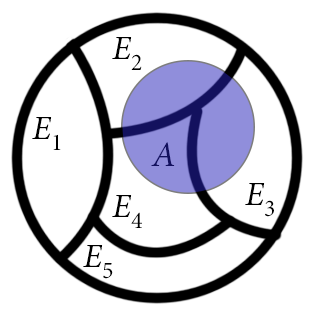
\includegraphics[width=3cm, height=3cm]{partition_rule}
\end{center}

Then for any event A: \(A = AE_1 \cup AE_2 ... \cup AE_k\). 

\begin{gather*}
p\left(A\right) = p\left(AE_1\right) + p\left(AE_2\right) + ... + p\left(AE_k\right) = \sum_{i = 1}^{k} \left(AE_i\right)
\end{gather*}

\begin{equation}
p\left(A\right) = \sum_{i = 1}^{k} p\left(E_i\right)p\left(A|E_i\right)
\end{equation}\\

Note that a often used partition of S is simply an event B and its complement \(\bar{B}\) since \(S = B \cup \bar{B}\).

\subsection{Bayes Rule}
Bayes rule is used to reverse the sign of conditional probability. For example, if we want to find \(p\left(A|B\right)\) but only have \(p\left(B|A\right)\), we can use bayes rule.

\begin{equation}
p(A|B) = \frac{p\left(AB\right)}{p\left(B\right)} = \frac{p\left(A\right)p\left(B|A\right)}{p\left(B\right)}
\end{equation}\\

\subsection{Example using all rules}
E.g Suppose 2\% of a population have a disease. A blood test for the disease gives a 5\% false positive rate and a 1\% false negative rate. What is the probability of a random person tests positive for the disease?\\

The first thing to note is that our sample space will contain the entire population of people. The second thing to note that is we have a partition of the sample space: all the people who have the disease and all the people who don't.\\

Let D = person has the disease. Let T = person tests positive for the disease. We know \(p\left(D\right) = 0.02, p(T|\bar{D}) = 0.05, p\left(\bar{T}|D\right) = 0.01\).\\

\(S = D \cup \bar{D}\). So by the partition rule and product rule:

\begin{align*}
p\left(T\right) &= p\left(D\right)p\left(T|D\right) + p\left(\bar{D}\right)p\left(T|\bar{D}\right)\\
&= 0.02(1 - 0.01) + 0.98(0.05) = 0.0688
\end{align*}

Suppose that someone tests positive. What is the probability they have the disease?\\

We want \(p\left(D|T\right)\). By Bayes rule:

\begin{align*}
p\left(D|T\right) &= \frac{p\left(D\right)p\left(T|D\right)}{p\left(T\right)}\\
&= \frac{0.02(1 - 0.01)}{0.0688}\\
&= 0.288
\end{align*}

\newpage

\section{Chapter 5}
We will now introduce the concept of random variables. As the name implies, random variables are random (i.e. they can take multiple values). The values that a random variable can take is called the range of the random variable.\\

Convention: X, Y, Z are often abbreviated as random variables and x, y, z are values they can take, respectively. Random variable is often abbreviated as r.v.\\

Random variables can be discrete or continuous. Discrete random variables are random variables who have a discrete range (finite or countably infinite). Continuous random variables are random variables who have a continuous range (uncountable infinite, like \(\mathbb{R}\)). For example a random variable that can take a value anywhere between 0 and 1.0 is continuous as there are uncountably infinite values in that range. This chapter will discuss discrete random variables.\\

The probability that X takes a value x is called the probability function of X:

\begin{equation}
f\left(x\right) = P\left(X = x\right) \;\;\; \forall x \in X
\end{equation}\\

The probability function of a random variable conforms to following axioms:

\begin{itemize}
\item \(0 \leq f\left(x\right) \leq 1\)
\item \(\sum\limits_{x \in X} f\left(x\right) = 1\)
\end{itemize}

The probability that X takes a value \(\leq\) x is called the cumulative distribution function of X:

\begin{equation}
F\left(x\right) = P\left(X \leq x\right) \;\;\; \forall x \in \mathbb{R}
\end{equation}\\

Note that cumulative distribution function is often abbreviated as c.d.f. Also note that it is defined for all real numbers.\\

The cumulative distribution function of a random variable conforms to following axioms:

\begin{itemize}
\item \(0 \leq F\left(x\right) \leq 1\)
\item \(\lim_{F\left(x\right)\to\infty} F\left(x\right) = 1\)
\item \(\lim_{F\left(x\right)\to{- \infty}} F\left(x\right) = 0\)
\item \(F\left(x\right)\) is non-decreasing
\end{itemize}

If \(x_o\) is the minimum then \(F\left(x_o\right) = f\left(x_o\right)\).

If \(x_o\) is the maximum then \(F\left(x_o\right) = 1\).

\(F\left(x\right)\) is non-decreasing because it is the sum of the values before it, that is, it is at least \(F\left(x - 1\right)\).\\

E.g. Graph the c.d.f for the following random variable X = number of 1's in 3 dice rolls:

\begin{center}
\begin{tabular}{|c|c|c|c|c|}
\hline
x & 0 & 1 & 2 & 3\\ \hline
\(f\left(x\right)\) & \(5^3/6^3\) & \(4\cdot(5^2)/6^3\) & \(15/6^3\) & \(1/6^3\)\\ 
\hline
\end{tabular}
\end{center}

\begin{gather*}
F\left(0\right) = P\left(X \leq 0\right) = f\left(0\right) = \frac{125}{216}\\
F\left(1\right) = P\left(X \leq 1\right) = f\left(0\right) + f\left(1\right) = \frac{5^3}{6^3} + \frac{4 \cdot 5^2}{6^3} = \frac{200}{216}\\
F\left(2\right) = P\left(X \leq 2\right) = f\left(0\right) + f\left(1\right) + f\left(2\right) = \frac{200}{216} + \frac{15}{6^3} = \frac{215}{216}\\
F\left(3\right) = P\left(X \leq 3\right) = 1
\end{gather*}
\begin{center}
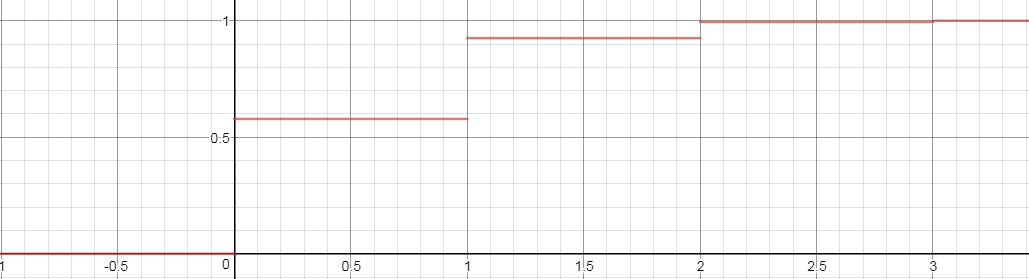
\includegraphics[width=15cm, height=5cm]{exampleF(x)}
\end{center}

So we see that \(F\left(x\right)\) is a right continuous step function with discontinuities at each value of x in X's range.\\

Also note that \(f\left(x\right) = F\left(x\right) - F\left(x - 1\right)\), that is, \(P\left(X = x\right) = P\left(X \leq x \right) - P\left(X \leq x - 1\right)\). 

\subsubsection{Discrete Uniform Random Variable}
Let X be a random variable that takes values in the range \(\{a, a + 1, ..., b\}\) such that each value is equally likely. Then we say X \emph{is a} discrete uniform random variable:

\begin{equation}
X \sim DU[a, b]
\end{equation}\\

E.g. Let X = value on die. Then \(X \sim DU[1, 6]\).\\

What is the probability function of X?

\begin{equation}
f\left(x\right) = P\left(X = x\right) = \frac{1}{b - a + 1}
\end{equation}\\

What is the cumulative distribution function of X?

\begin{equation}
F\left(x\right) = P\left(X \leq x\right) = 
	\begin{cases} 
      0 & x < a \\
      1 & x > b \\
      \sum\limits_{i = a}^{\left \lfloor{x}\right \rfloor} \frac{1}{b - a + 1} = \frac{\left \lfloor{x}\right \rfloor - a + 1}{b - a + 1} & a \leq x \leq b
	\end{cases}
\end{equation}\\

Note that, in the discrete uniform case, the cumulative distribution function has "jumps" of equal heights.

\subsubsection{Hypergeometric Random Variable}
Suppose you have \(N\) objects, \(r\) of which are successes and \(N - r\) are fails. Suppose we draw \(n\) objects without replacement and order doesn't matter. Let X be a random variable that counts the number of successes in those \(n\) objects. Then we say X \emph{is a} hypergeometric random variable:

\begin{equation}
X \sim Hyper(N, r, n)
\end{equation}\\

E.g. In lotto 6/49 six numbers are drawn from \(\{1, 2, ..., 49\}\) to be winning numbers. Players draw 6 numbers\footnote{"Draw" often implies without replacement and order doesn't matter.}. Let X = number of winning numbers a player draws. Then \(X \sim Hyper(49, 6, 6)\).\\

What is the probability function of X?

\begin{equation}
f\left(x\right) = p\left(\text{we draw $x$ successes \emph{and} $n - x$ failures}\right) = \frac{{r \choose x}{{N - r} \choose {n - x}}}{{{N} \choose {n}}}
\end{equation}\\

What is the range of X?

The largest number of successes we can draw is either limited by how many successes there are, \(r\), or how many objects were picking, \(n\). The smallest number of successes we draw is either limited by 0 or the maximum number of fails we can draw, \(n - (N - r)\).\\

For example, suppose N = 49, r = 6, n = 3. The highest number of successes we can draw is 3. Now suppose N = 49, r = 6, n = 9. The highest number of successes we can draw is 6.\\

Similarly, suppose N = 49, r = 6, n = 6. The lowest number of successes we can draw 0. Now suppose N = 10, r = 6, n = 6. The lowest number of successes we can get is 2.\\

In general, the range is Max(\(0, n - (N - r)) \leq x \leq \) Min(\(n ,r\)).

Unfortunately there is no closed form of the cumulative distribution function for hypergeometric random variables.

\subsubsection{Binomial Random Variable}
The binomial random variable relies on a concept known as bernoulli trials. Bernoulli trials are trials of an experiment that conform under the following axioms:
\begin{itemize}
\item Trials are independent.
\item Each trial is either a success or a failure.
\item The probability of success, p, is constant.
\end{itemize}

Suppose there are \(n\) trials and the probability of success is \(p\). Let X = number of successes in those \(n\) trials. Then we say X is a binomial random variable:

\begin{equation}
X \sim Bin(n, p)
\end{equation}

E.g. Flipping 10 coins. Let X = number of heads in those 10 flips. Then \(X \sim Bin(10, 0.5)\).\\

What is the probability function of X?
\begin{equation}
f\left(x\right) = p\left(\text{we get $x$ successes \emph{and} $n - x$ failures}\right) = {{n} \choose {x}} p^x (1 - p)^{n - x}
\end{equation}\\

Note that \(p^x (1 - p)^{n-x}\) is the probability of getting \(x\) successes and \(n - x\) fails in a row. That is, \(\underbrace{p p ... p}_\text{x times}\) \(\underbrace{(1 - p) (1 - p) ... (1 - p)}_\text{n - x times}\). In reality, those successes and failures can occur in any order, as long as they add up to \(x\) successes and \(n - x\) failures. So we need to account for all the ways to place \(x\) successes in \(n\) trials (with the rest of the trials being failures) \({{n} \choose {x}}\).\\

What is the range of X?

The smallest number of successes we get can get in \(n\) trials is 0. The largest number of successes we can get is \(n\). So the range is \(\{0, 1, 2, 3, ..., n\}\).\\

Unfortunately there is no closed form of the cumulative distribution function for binomial random variables.

\subsubsection{Approximation of Hypergeometric using Binomial}
Suppose we have \(N\) objects, \(r\) of which are successes and \(N - r\) are fails. Suppose we draw \(n\) objects without replacement and order doesn't matter and \(n << N\). That is, the number of objects that were drawing is much smaller than the total number of objects. Let X = number of successes in \(n\) objects.\\

Then, whether we sample with or without replacement doesn't really matter because it is extremely unlikely to get the same object twice.\\

If we treat the problem without replacement then \(X \sim Hyper(N, r, n)\).\\

If we treat the problem with replacement then \(X \sim Bin(n, \frac{r}{N})\).\\

\subsubsection{Negative Binomial Random Variable}
Suppose there are n trials and the probability of success is p. Let X = number of failures before the kth success. Then we say X is a negative binomial random variable:

\begin{equation}
X \sim NB(k, p)
\end{equation}\\

E.g. Roll a dice until you roll 6 1's. Let X = number of non 1's before the 6th 1, \(X \sim NB(6, \frac{1}{6})\).\\

E.g. Suppose the probability of passing a course for a student is p and courses are independent. Let X = number of failed courses before passing 40 courses, \(X \sim NB(40, p)\).\\

What is the probability function of X?
\begin{align*}
f\left(x\right) &= p\left(\text{$x$ fails before kth success}\right)\\
&= p\left(\text{$x$ fails \text{\emph{and}} k - 1 successes before kth success}\right)
\end{align*}

\[
\underbrace{
\begin{tabular}{|c|c|c|c|c|c|c|c|c|}
	\hline \_ & \_ & \_ & \_ & \_ & \_ & ... & \_ \\ \hline
\end{tabular}
}_\text{x fails and k - 1 successes}
\underbrace{S}_\text{kth success}
\]

\begin{equation}
f\left(x\right) = {{x + k - 1} \choose {x}}p^k (1 - p)^x = {{x + k - 1} \choose {k - 1}}p^k (1 - p)^x
\end{equation}\\

Note that \(p^k (1 - p)^{x}\) is the probability of getting \(k\) successes and \(x\) fails in a row. That is, \(\underbrace{p p ... p}_\text{k times}\) \(\underbrace{(1 - p) (1 - p) ... (1 - p)}_\text{x times}\). In reality, those successes and failures can occur in any order, as long as they add up to \(x\) fails and \(k - 1\) successes. So we need to account for all the ways to place \(x\) fails in \(x + k - 1\) trials (with the rest of the trials being successes) \({{x + k - 1} \choose {x}}\).\\

What is the range of X?

The smallest number of fails before the kth success is 0. However, in theory, there is no maximum number of fails before the kth success. So the range is \(\{0, 1, 2, 3, ...\}\).

E.g. Suppose a startup is looking for 5 investors. Each investor independently agrees with probability 0.2. Founders ask one investor at a time until 5 investors say yes. How many investors do they ask?\\

Let X = number of investors that say no before the 5th investor says yes. Then \(X \sim NB(5, 0.2)\). Let Y = total number of investors they ask. Then \(Y = X + 5\).

\begin{align*}
f\left(x\right) = P\left(X = x\right)
&= P\left(Y - 5 = x\right)\\
&= P\left(Y = x + 5\right) = {{x + 5 + 5 - 1} \choose {x + 5}}p^5 (1 - p)^{x + 5}\\
&= {{x - 9} \choose {x + 5}}p^5 (1 - p)^{x + 5}
\end{align*}

E.g. Suppose someone sends a bit stream of 0's and 1's over a noisy connection. The probability that a bit gets flipped is 0.01. Find the probability it takes 50 bits to observer 5 errors.\\

Let X = number of non-flipped bits before the 5th error. Then \(X \sim NB(5, 0.01)\).

\begin{align*}
p\left(\text{takes 50 bits to observe 5 errors}\right)
&= P\left(X = 45\right)\\
&= {{49} \choose {4}}0.01^5 (1 - 0.01)^{45}
\end{align*}

\subsubsection{Geometric Random Variable}
The geometric random variable is just a special case of the negative binomial random variable. Suppose there are n trials and the probability of success is p. Let X = number of fails before the first success. Then we say X is a geometric random variable:

\begin{equation}
X \sim Geo(p)
\end{equation}\\
 
What is the probability function of X?
\begin{equation}
f\left(x\right) = p\left(\text{$x$ fails before first success}\right) = p(1 - p)^x
\end{equation}\\

What is the range of X?

The smallest number of fails before a success is 0. However, just like the negative binomial random variable, in theory, there is no maximum number of fails before a success. So the range is \(\{0, 1, 2, 3, ...\}\).\\

What is cumulative distribution function of X?

\begin{align*}
F\left(x\right) = P\left(X \leq x\right)
&= 1 - P\left(X \geq x + 1\right)\\
&= 1 - (f\left(x + 1\right) + f\left(x + 2\right) + ...)\\
&= 1 - (p(1 - p)^{x + 1} + p(1 - p)^{x + 2} + ...)\\
&= 1 - \frac{p(1 - p)^{x + 1}}{1 - (1 - p)} \text{by geometric series}\\
&= 1 - (1 - p)^{x + 1}
\end{align*}\\

E.g. Suppose a safe has a 10 digit code. You randomly try keys with replacement (don't keep track of keys you already tried). What is the probability of cracking the safe in 11 tries or fewer?\\

Let X = number of failed attempts before unlocking the safe. Then \(X \sim Geo(\frac{1}{10^{10}})\).

\begin{align*}
F\left(11\right) = 1 - (1 - \frac{1}{10^{10}})^{11}
\end{align*}

\subsubsection{Poisson Random Variable}
The poisson random variable relies on a concept known as a poisson process. A poisson process is a process where events occur randomly with continuous time and:
\begin{itemize}
\item The number of events in non-overlapping time intervals are independent
\item Events occur one at a time (probability of two or more events occurring at the same time is 0) 
\item Events occur at a constant average rate, \(\lambda\)
\end{itemize} 

Suppose you have a poisson process and rate \(\lambda\) and Let X = number of events that occur in \(t\) units of time. Then we say X is a poisson random variable:

\begin{equation}
X \sim Poi(\mu = \lambda t)
\end{equation}\\

Note: Make sure \(\lambda\) and \(t\) are measured in the same time units.\\

The poisson process is often used to model:
\begin{itemize}
\item Births in a large population
\item Number of requests to a server
\item Number of collisions in a nuclear reaction
\item Traffic accidents
\end{itemize}

The probability function of X is:
\begin{equation}
f\left(x\right) = \frac{e^{-\mu}\mu^x}{x!}
\end{equation}\\

What is the range of X?

The smallest number of events that occur in \(t\) units of time is 0. There is no maximum so the range is \(\{0, 1, 2, 3, ...\}\).\\

E.g. Server requests come according to a poisson process with rate 100 \(\frac{requests}{minute}\). Find the probability of 1 request and 1 second.\\

Let X = number of requests that come in one second. Then \(X \sim Poi(\frac{\text{100 requests}}{\text{60 secs}} * 1 \text{ sec}) = Poi(\frac{100}{60})\).

\begin{align*}
P\left(X = 1\right) = \frac{e^{-\frac{100}{60}} \frac{100}{60}^1}{1!}
\end{align*}

\subsubsection{Approximation of Binomial using Poisson}
Suppose you have \(n\) trials and the probability of success is \(p\). Let X = number of successes in those \(n\) trials. Suppose also that \(n \rightarrow \infty\) and \(p \rightarrow 0\). That is, the number of trials goes to infinity and the probability of success goes to 0. \\

Then X can be modeled by a poisson random variable: \(X \sim Poi(\mu = np)\).\\

Lets prove this by showing that if we impose the conditions of \(n \rightarrow \infty\) and \(p \rightarrow 0\) on the binomial random variable, it becomes the poisson random variable:

\begin{align*}
f\left(x\right) &= \lim_{n \rightarrow \infty} {{n} \choose {x}} p^x (1 - p)^{n - x}\\
&= \lim_{n \rightarrow \infty} \frac{n!}{x!(n - x)!} \left(\frac{\mu}{n}\right)^x \left(1 - \frac{\mu}{n}\right)^{n - x}\\
&= \lim_{n \rightarrow \infty} \frac{n(n - 1)(n - 2)...(n - x + 1)}{x!} \frac{\mu^x}{n^x} \left(1 - \frac{\mu}{n}\right)^{n - x}\\
&= \frac{\mu^x}{x!} \lim_{n \rightarrow \infty} \frac{n(n - 1)(n - 2)...(n - x + 1)}{n^x} \left(1 - \frac{\mu}{n}\right)^{n - x}\\
&= \frac{\mu^x}{x!} \lim_{n \rightarrow \infty} \frac{n}{n} \cdot \frac{n - 1}{n} \cdot \frac{n - 2}{n} ... \frac{n - x + 1}{n} \left(1 - \frac{\mu}{n}\right)^{n - x}\\
&= \frac{\mu^x}{x!} \lim_{n \rightarrow \infty} \left(1 - \frac{\mu}{n}\right)^{n - x}
\end{align*}

Recall from calculus: \(\lim_{n \rightarrow \infty} \left(1 + \frac{a}{n}\right) = e^a\).

\begin{align*}
f\left(x\right) = \frac{e^{-\mu}\mu^x}{x!}
\end{align*}

\subsubsection{Important Series}
Memorize the following:\\

Geometric Series: If \(\vert r \vert < 1\):
\begin{align*}
\sum_{k = 0}^{\infty} ar^k = \frac{a}{1 - r}\\
\sum_{k = 0}^{n} ar^k = \frac{a(1 - r)^{n + 1}}{1 - r}
\end{align*}

Binomial Theorm:
\begin{align*}
(1 + x)^n = \sum_{k = 0}^{n} {{n} \choose {k}} x^k
\end{align*}

Hypergeometric Identity:
\begin{align*}
{{a + b} \choose {n}} = \sum_{k = 0}^{n} {{a} \choose {k}} {{b} \choose {n - k}}
\end{align*}

Exponential Series:
\begin{align*}
e^x = \sum_{k = 0}^{\infty} \frac{x^k}{k!}
\end{align*}

\newpage

\section{Chapter 6}
Not covered in STAT 230.

\newpage

\section{Chapter 7}
Knowing the entire distribution is nice but sometimes we want a few numbers that summarize the distribution.

\subsubsection{Summarizing Data}
E.g. Let X = number of kids in a family.

Suppose a group was surveyed and it was found that 5 families had 1 kid, 12 families had 2 kids, 7 families had 3 kids and 2 families had 4 kids.\\

Sample mean (denoted \(\overline{X}\)): The sample mean of a random variable is the average of the random variable. It is called the sample mean because it is often different for every sample. The sample mean of X is the average number of kids in a family.

\begin{align*}
\overline{X} &= \frac{\text{Total number of kids}}{\text{Total number of families}}\\
&= \frac{1 \cdot 5 + 2 \cdot 12 + 3 \cdot 7 + 4 \cdot 2 }{5 + 12 + 7 + 2}\\
&= 2.23
\end{align*}\\

Median: The median is also called the middle value. The median of a random variable is the middle sorted value. The median of X is the middle value if we sorted the number of kids from lowest to highest. Notice that X has two middle values since it is an even number.

\begin{align*}
Median(X) = \frac{2 + 2}{2} = 2
\end{align*}\\

Mode: The mode is the most common value. The mode of X is the most common number of kids for a family to have.

\begin{align*}
Mode(X) = 2
\end{align*}

\subsubsection{Expected Value}
The expected value of a random variable is its mean, that is, the average value of the random variable.\\

Recall from the above example that the sample mean of X, the number of kids in a family is:
\begin{align*}
\overline{X} &= \frac{\text{Total number of kids}}{\text{Total number of families}}\\
&= \frac{1 \cdot 5 + 2 \cdot 12 + 3 \cdot 7 + 4 \cdot 2 }{5 + 12 + 7 + 2}\\
&= \frac{1 \cdot 5 + 2 \cdot 12 + 3 \cdot 7 + 4 \cdot 2 }{26}\\
&= 1.8
\end{align*}

We can rearrange this expression to get a much simpler form:
\begin{align*}
\overline{X} &= 1 \cdot \frac{1}{26} + 2 \cdot \frac{12}{26} + 3 \cdot \frac{7}{26} + 4 \cdot \frac{2}{26}\\
&= \sum_{x = 1}^4 x f\left(x\right)
\end{align*}

So we can think of the the sample mean (and thus the mean) as the weighted average of x with the weights being the probabilities.\\

In general, for a random variable X, the expected value of X is:
\begin{equation}
E[X] = \sum_{\text{all x}} xf\left(x\right) = \mu
\end{equation}\\

Just like the sample mean, we can think of the expected value of X as the weighted average of x with the weights being the probabilities that x occurs.\\

E.g. Let X = number of kids in a family with the probability function:\\

\begin{tabular}{|c|c|c|c|c|c|}
\hline
X & 1 & 2 & 3 & 4 & 5\\ 
\hline
$f\left(x\right)$ & 0.43 & 0.4 & 0.12 & 0.04 & 0.01\\
\hline
\end{tabular}\\

Suppose we have another function, \(g\left(X\right)\), that determines the tax credit for a family with x amount of kids where \(g\left(X\right) = 1000 + 250X\). What is the average tax credit for a family, \(E[g\left(X\right)]\)?\\

Just like \(E[X]\) is the weighted average of x with the weights being the probabilities that x occurs, \(E[g\left(X\right)]\) is the weighted average of g(x) with the weights being the probabilities that x occurs.

\begin{align*}
E[g\left(X\right)] = (\text{tax credit for 1 kid})(\text{probability of having 1 kid}) + \\
(\text{tax credit for 2 kid})(\text{probability of having 2 kid}) + \\
(\text{tax credit for 3 kid})(\text{probability of having 3 kid}) + \\
(\text{tax credit for 4 kid})(\text{probability of having 4 kid})\\
= 1250 \cdot 0.43 + 1500 \cdot 0.4 + 1750 \cdot 0.12 + 2000 \cdot 0.04 + 2250 \cdot 0.01 = 1450
\end{align*}

However, notice that we could have gotten \(E[g\left(X\right)]\) in a much easier way:

\begin{align*}
E[g\left(X\right)] &= E[1000 + 250X] \\
&= 1000 + 250E[X]\\
&= 1000 + 250 \cdot 1.8 = 1450
\end{align*}

E.g. Now suppose \(g\left(X\right) = \frac{2000}{X}\). What is the average tax credit for a family, \(E[g\left(X\right)]\)?

\begin{align*}
E[g\left(X\right)] = \frac{2000}{1} \cdot 0.43 + \frac{2000}{2} \cdot 0.4 + \frac{2000}{3} \cdot 0.12 + \frac{2000}{4} \cdot 0.04 + \frac{2000}{5} \cdot 0.01 = 1364
\end{align*}

Could we have gotten \(E[g\left(X\right)]\) in a much easier way?

\begin{align*}
E[g\left(X\right)] &= E\left[\frac{2000}{X}\right] \\
&= \frac{2000}{E[X]}\\
&= \frac{2000}{1.8} = 1111 \neq 1364
\end{align*}

The reason why it worked in the first example is because expectation is a linear operator. That is, \(E[aX + b] = aE[X] + b\).\\

Lets prove this using the definition of expectation:

\begin{align*}
E[aX + b] &= \sum_{\text{all x}} (ax + b)f\left(x\right)\\
&= \sum_{\text{all x}} axf\left(x\right) + \sum_{\text{all x}} bf\left(x\right)\\
&= a\sum_{\text{all x}} xf\left(x\right) + b\sum_{\text{all x}} f\left(x\right)\\
&= aE[X] + b
\end{align*}\\

In general:
\begin{align}
E[aX + b] = aE[X] + b\\
E[g\left(X\right)] = g\left(E[X]\right) \text{ if } g\left(X\right) \text{ linear}
\end{align}

\newpage

\subsubsection{Expectations of Named Distributions}
Suppose \(X \sim Bin(n, p)\). What is \(E[X]\)?

\begin{align*}
E[X] &= \sum_{x = 0}^n x f\left(x\right)\\
&= \sum_{x = 0}^n x {{n} \choose {x}} p^x (1 - p)^{n - x}\\
&= \sum_{x = 1}^n \frac{xn!}{x!(n - x)!} p^x (1 - p)^{n - x}\\
&= \sum_{x = 1}^n \frac{n!}{(x - 1)!(n - x)!} p^x (1 - p)^{n - x}\\
&= \sum_{x = 1}^n \frac{n(n - 1)!}{(x - 1)!((n - 1) - (x - 1))!} p^x (1 - p)^{n - x}\\
&= \sum_{x = 1}^n \frac{n(n - 1)!}{(x - 1)!((n - 1) - (x - 1))!} pp^{x - 1} (1 - p)^{(n - 1) - (x - 1)}\\
&= np \sum_{x = 1}^n {{n - 1} \choose {x - 1}} p^{x - 1} (1 - p)^{(n - 1) - (x - 1)} \text{ Let } y = x - 1\\
&= np \underbrace{\sum_{y = 0}^{n - 1} {{n - 1} \choose {y}} p^{y} (1 - p)^{(n - 1) - y}}_\text{This is the probability function of $Y \sim Bin(n - 1, p)$ summed over its range}\\
&= np
\end{align*}

Note that the result also makes logical sense. If we have \(n\) trials and the probability of success is \(p\). The expected number of successes should be \(np\). It should be proportional to \(n\) and \(p\). As the number of trials increases so does the expected number of successes. As the probability of success increases so does the expected number number of successes.\\

\newpage

Suppose \(X \sim Poi(\mu)\). What is \(E[X]\)?

\begin{align*}
E[X] &= \sum_{x = 0}^{\infty} xf\left(x\right)\\
&= \sum_{x = 0}^{\infty} x\frac{e^{-\mu}\mu^x}{x!}\\
&= \sum_{x = 1}^{\infty} \frac{e^{-\mu}\mu^x}{(x - 1)!} \text{ Let } y = x - 1\\
&= \mu \underbrace{\sum_{y = 0}^{\infty} \frac{e^{\mu}\mu^y}{y!}}_\text{This is the probability function of $Y \sim Poi(\mu)$ summed over its entire range}\\
&= \mu
\end{align*}

Note that the result also makes logical sense. If we had a poisson process with rate \(\lambda\) and were counting the number of events in \(t\) units of time, it makes sense that the expected number of events is \(\lambda t\). It should be proportional to \(\lambda\) and \(t\). As the average rate that events occur increases so does the expected number of events. As we watch for longer periods of time, the expected number of events increases.\\

The expected value for other named distributions can be found on the formula sheet.

\subsubsection{Variance}
We want a way to measure how spread out a distribution is around its mean value. That is, we want to know how much it \emph{varies} around its mean value. The variance of a random variable X is defined to be:

\begin{equation}
Var\left(X\right) = E[(X - E[X])^2] = \sigma^2
\end{equation}\\

The variance of a random variable X is the average squared distance from the mean. The reason why we  define the variance to be the squared distance from the mean is because we want to work with the absolute value. However, we cannot define variance to be the absolute value because the function is undefined at x = 0, which is troublesome to deal with. Also note that the variance is always non-negative.\\

An alternate definition of variance can be derived if we simplify:

\begin{align*}
Var\left(X\right) &= E[(X - E[X])^2]\\
&= E[X^2 - 2XE[X] + E[X]^2]\\
&= E[X^2] -2E[X]E[X] + E[X]^2\\
&= E[X^2] -2E[X]^2 + E[X]^2\\
&= E[X^2] - E[X]^2
\end{align*}

So the variance can also be defined as follows:

\begin{equation}
Var\left(X\right) = E[X^2] - E[X]^2
\end{equation}

Recall to find \(E[X^2]\):
\begin{align*}
E[X^2] = \sum_{\text{all x}} x^2 f\left(x\right)
\end{align*}\\

E.g. Let X = time to complete coding with the probability function:\\

\begin{tabular}{|c|c|c|c|c|}
\hline
X & 10 & 12 & 20 & 22\\ 
\hline
$f\left(x\right)$ & 0.72 & 0.08 & 0.18 & 0.02\\
\hline
\end{tabular}\\

What is the \(Var\left(X\right)\)?\\

Recall \(Var\left(X\right) = E[X^2] - E[X]^2\).

\begin{align*}
E[X^2] &= \sum_{\text{all x}}x^2 f\left(x\right)\\
&= 10^2 \cdot 0.72 + 12^2 \cdot 0.08 + 20^2 \cdot 0.18 + 22^2 \cdot 0.02\\
&= 165.2 \text{ minute}^2
\end{align*}

\begin{align*}
E[X] &= \sum_{\text{all x}} xf\left(x\right)\\
&= 10 \cdot 0.72 + 12 \cdot 0.08 + 20 \cdot 0.18 + 22 \cdot 0.02\\
&= 12.2
\end{align*}

\begin{align*}
Var\left(X\right) = 165.5 - 12.2^2 = 16.36 \text{ minute}^2
\end{align*}

Notice that the variance is always in squared units of X. This can be difficult to interpret so we have another unit of measurement, called the standard deviation. The standard deviation of a random variable X is:

\begin{equation}
SD\left(X\right) = \sqrt{Var\left(X\right)} = \sigma
\end{equation}\\

The standard deviation of X in the previous example is:
\begin{align*}
Var\left(X\right) = \sqrt{16.36} = 4.04 \text{ minutes}
\end{align*}

Question: What is \(Var\left(Y = aX + b\right)\)?

\begin{align*}
Var\left(Y = aX + b\right) &= E[(Y - E[Y])^2]\\
&= E[(aX + b - E[aX + b])^2\\
&= E[(aX + b - aE[X] - b)^2]\\
&= E[(aX - aE[X])^2]\\
&= E[a^2(X - E[X])^2]\\
&= a^2 E[(X - E[X])^2]\\
&= a^2 Var\left(X\right)
\end{align*}

In general:
\begin{equation}
Var\left(aX + b\right) = a^2 Var\left(X\right)
\end{equation}\\

Notice that b does not affect the variance. The reason why is because shifting the distribution by a constant doesn't affect the spread of the data at the mean.

\subsubsection{Variances of Named Distributions}
Suppose \(X \sim Bin(n, p)\). What is \(Var\left(X\right)\)?

\begin{align*}
Var\left(X\right) &= E[X^2] - E[X]^2\\
&= E[X^2 - X + X] - E[X]^2\\
&= E[X(X - 1) + X] - E[X]^2\\
&= E[X(X - 1)] + E[X] - E[X]^2
\end{align*}
\begin{align*}
E[X(X - 1)] &= \sum_{x = 0}^{n} x(x - 1)f\left(x\right)\\
&= \sum_{x = 2}^{n} x(x - 1) \frac{n!}{x! (n - x)!} p^x (1 - p)^{n - x}\\
&= \sum_{x = 2}^{n} \frac{n(n - 1)(n - 2)!}{(x - 2)! (n - x)!} p^x (1 - p)^{n - x}\\
&= \sum_{x = 2}^{n} \frac{n(n - 1)(n - 2)!}{(x - 2)! ((n - 2) - (x - 2))!} p^2 p^{x - 2} (1 - p)^{(n - 2) - (x - 2)}\\
&= n(n - 1)p^2 \sum_{x = 2}^{n} \frac{(n - 2)!}{(x - 2)! ((n - 2) - (x - 2))!} p^{x - 2} (1 - p)^{(n - 2) - (x - 2)}\\
&= n(n - 1)p^2 \sum_{x = 2}^{n} {{n - 2} \choose {x - 2}} p^{x - 2} (1 - p)^{(n - 2) - (x - 2)} \text{ Let } y = x - 2 \\
&= n(n - 1)p^2 \underbrace{\sum_{y = 0}^{n - 2} {{n - 2} \choose y} p^{y} (1 - p)^{(n - 2) - y}}_\text{This is the probability function of $Y \sim Bin(n - 2, p)$ summed over its entire range}\\
&= n(n - 1)p^2
\end{align*}

\begin{align*}
Var\left(X\right) &= n(n - 1)p^2 + np - (np)^2\\
&= n^2 p^2 - np^2 + np - n^2 p^2\\
&= -np^2 + np\\
&= np (1 - p)
\end{align*}

Suppose \(X \sim Poi(\mu)\). We find that the variance of X is: \(Var\left(X\right) = \mu\).\\

The variance for other named distributions can be found on the formula sheet.

\section{Chapter 8}
We will now introduce the concept of continuous random variables. Continuous random variables are random variables with a uncountably infinite range.\\

E.g. Let X = temperature on a given day. Given infinite precision, there are uncountably infinite possibilities.\\

E.g. Let Y = heights of a population.\\

In general, if the thing that are you are modeling can be measured with infinite precision, it can be modeled by a continuous random variable.\\

What is the probability function for a continuous random variable, X?

Since the range is uncountably infinite, \(f\left(x\right) = P\left(X = x\right) = 0,  \forall x\). Therefore the probability function is useless when dealing with continuous random variables.\\

The cumulative distribution function for a continuous random variable is the same, \(F\left(x\right) = P\left(X \leq x\right)\). However, \(P\left(a \leq X \leq b\right) = P\left(a < X \leq b\right) = P\left(a \leq X < b\right) = P\left(a < X < b\right) = F\left(b\right) - F\left(a\right)\), since \(P\left(X = a\right) = P\left(X = b\right) = 0\). That is, the end points don't matter when dealing with continuous random variables.\\

Also note that the cumulative distribution function for a continuous random variable is actually continuous. Recall that the c.d.f for discrete random variables had discontinuities at each value of x where the heights would correspond to \(f\left(x\right)\). However, since \(f\left(x\right) = 0, \forall x\), each of those jump heights are now equal to 0 and the c.d.f is a continuous function.\\

To describe continuous random variables, we define another function called the probability density function that is the derivative of the cumulative distribution function, \(f\left(x\right) = F'\left(x\right)\). The properties of \(f\left(x\right)\) is as follows:
\begin{itemize}
\item \(f\left(x\right) \geq 0\) since \(F\left(x\right)\) is a non-decreasing function. Note that the p.d.f can be bigger than 1 so it should not be interpreted as a probability
\item $$F\left(x\right) = \int_{- \infty}^{x} f\left(x\right)dx$$
\item $$P\left(a \leq X \leq b\right) = F\left(b\right) - F\left(a\right) = \int_{a}^{b} f\left(x\right)dx$$
\item $$\int_{\infty}^{\infty} f\left(x\right) = 1$$
\end{itemize}

E.g. Suppose you have a continuous random variable on range 0 - 1:
\begin{align*}
F\left(x\right) =
	\begin{cases} 
      0 & x < 0 \\
      1 & x > 1 \\
      x^2 & 0 \leq x \leq 1
	\end{cases}
\end{align*}
Find $f\left(x\right)$, $P\left(X = 0.25\right)$, $P\left(X \leq 0.25\right)$:

\begin{align*}
P\left(X = 0.25\right) = 0\\
f\left(x\right) = 
	\begin{cases}
	2x & 0 \leq x \leq 1\\
	0 & elsewhere
	\end{cases}\\
P\left(X \leq 0.25\right) = F\left(0.25\right) = 0.25^2\\
P\left(X \leq 0.25\right) = \int_{0}^{0.25} 2x dx = x^2 \vert_{0}^{0.25} = 0.25^2
\end{align*}

\subsubsection{Expected Value and Variance}
Rule of thumb: when working with continuous random variables, replace \(\sum\) with \(\int_{-\infty}^{\infty}\) and use the probability density function instead of the probability function.

\begin{align}
E[X] = \int_{-\infty}^{\infty} x f\left(x\right) dx\\
E[g\left(X\right)] = \int_{-\infty}^{\infty} g\left(x\right) f\left(x\right) dx\\
Var\left(X\right) = \int_{-\infty}^{\infty} x^2 f\left(x\right) dx - \left(\int_{-\infty}^{\infty} x f\left(x\right) dx\right)^2
\end{align}

\subsubsection{Percentiles}
The pth percentile of a random variable in the value \(x_p\) such that \(P\left(X \leq x_p\right) = p\).\\

E.g. Suppose X has the p.d.f function: \(f\left(x\right) = cx^2, 0 < x < 2\) and 0 otherwise. Find c and \(E[X]\).\\

\begin{align*}
\int_{0}^{2} cx^2 dx = 1 = c \left[\frac{x^3}{3}\right]_{0}^{2} = \frac{8c}{3} = 1 \rightarrow c = \frac{3}{8}\\
E[X] = \int_{0}^{2} x \frac{3}{8} x^2 dx = \frac{3}{8} \left[\frac{x^4}{4}\right]_{0}^{2} = 1.5
\end{align*}

\subsubsection{Uniform Random Variable}
Let X be a continuous random variable that takes real values between (a, b) such that all sub-intervals of a fixed length are equally likely. Then we say X is a uniform random variable:

\begin{equation}
X \sim U(a, b)
\end{equation}\\

Note that the uniform random variable is not defined as: every value in (a, b) is equally likely because \(P\left(X = x\right) = 0, \forall x\). So, if we did define it that way, every continuous random variable would be a uniform random variable.\\

What is the probability density function?

Since every sub-interval of fixed length is equally likely, \(F\left(x\right)\) grows linearly. So \(f\left(x\right) = F'\left(x\right) = c\) (constant).

\begin{align*}
\int_{a}^{b} c dx = 1 = c (b - a) \rightarrow f\left(x\right) = c = \frac{1}{b - a}\\
f\left(x\right) = 
	\begin{cases}
	\frac{1}{b - a} & a < x < b\\
	0 & otherwise
	\end{cases}
\end{align*}

What is the cumulative distribution function?

\begin{align*}
F\left(x\right) &= \int_{-\infty}^{x} f\left(x\right) dx = \int_{a}^{x} \frac{1}{b - a} dx = \frac{1}{b - a} x \vert_{a}^{x} = \frac{x - a}{b - a}\\
&= 
	\begin{cases}
	\frac{x - a}{b - a} & a < x < b\\
	0 & x < a\\
	1 & x > b
	\end{cases}
\end{align*}

What is the expected value and variance?

\begin{align*}
E[X] &= \int_{-\infty}^{\infty} x f\left(x\right) dx = \int_{a}^{b} x \frac{1}{b - a} dx\\
&= \frac{1}{b - a} \left[\frac{x^2}{2}\right]_{a}^{b} = \frac{b^2 - a^2}{2(b - a)}\\
&= \frac{b + a}{2}\\
Var\left(X\right) &= E[X^2] - E[X]^2 = ... = \frac{(b - a)^2}{12}
\end{align*}\\

E.g. Suppose there is a spinner that can land on a value been 0 and 4. Let X = value spinner lands on. Then \(X \sim U(0, 4)\), \(f_x \left(x\right) = \frac{1}{4}\), 0 otherwise, \(F_x \left(x\right) = \frac{x}{4}\), \(0 < x < 4\). Let Y = \(\frac{1}{X}\). Find the p.d.f of Y.\\

What is the range of Y?

We know the range of X is (0, 4). So the range of Y is (\(-\infty, \frac{1}{4}\)).

\begin{align*}
F_Y \left(y\right) = P\left(Y \leq y \right) &= P\left(\frac{1}{X} \leq y\right)\\
&= P\left(X \geq \frac{1}{y}\right) = 1 - P\left(X < \frac{1}{y}\right)\\
&= 1 - P\left(X \leq \frac{1}{y}\right) = 1 - F_x \left(\frac{1}{y}\right)
\end{align*}

\begin{align*}
f_Y \left(y\right) &= F_Y '\left(y\right) = \frac{d}{dy} \left(1 - F_x \left(\frac{1}{y}\right)\right)\\
&= -F_x \left(\frac{1}{y}\right) * -\frac{1}{y^2} = \frac{1}{4y} \frac{1}{y^2} = \frac{1}{4y^2}, 0 < \frac{1}{y} < 4\\
&= \frac{1}{4y^2}, 0 < 1 < 4y \rightarrow y > \frac{1}{4}
\end{align*}

\begin{align*}
f_Y \left(y\right) = 
	\begin{cases}
	\frac{1}{4y^2} & y > \frac{1}{4}\\
	0 & otherwise
	\end{cases}
\end{align*}

\subsubsection{Exponential Random Variable}
Suppose you have a poisson process with rate \(\lambda\). Instead of counting how many times an event occurs in a fixed amount of time (which is discrete), we count the waiting time until the next event happens. Let X be the waiting time until the next event. Then we say X has a exponential distribution:

\begin{equation}
X \sim Exp(\theta = \frac{1}{\lambda})
\end{equation}\\

What is the cumulative distribution function of X?
\begin{align*}
F\left(x\right) = P\left(X \leq x\right) &= 1 - P\left(X \geq x\right)\\
&= 1 -  p\left(\text{time until the next event occurs is $>$ x}\right)\\
&= 1 -  p\left(\text{no events between 0 and x}\right)
\end{align*}\\

Let Y = number of events between 0 and x. Then Y is a discrete random variable: \(Y \sim Poi(\lambda x)\).

\begin{align*}
F\left(x\right) &= 1 -  p\left(\text{no events between 0 and x}\right)\\
&= 1 - \frac{e^{-\lambda x} (\lambda x)^0}{0!}\\
&= 1 - e^{\lambda x} = 1 - e^{- \frac{x}{\theta}}\\
&= 
	\begin{cases}
	1 - e^{- \frac{x}{\theta}} & x > 0\\
	0 & otherwise
	\end{cases}
\end{align*}\\

What is the probability density function of X?
\begin{align*}
f\left(x\right) = F' \left(x\right) =
	\begin{cases}
	\frac{1}{\theta} e^{-\frac{x}{\theta}} & x > 0\\
	0 & otherwise
	\end{cases}
\end{align*}

What is the expected value of X?
\begin{align*}
E[X] &= \int_{-\infty}^{\infty} x f\left(x\right) dx = \int_{0}^{\infty} x f\left(x\right) dx\\
&= \int_{0}^{\infty} \frac{x}{\theta} e^{-\frac{x}{\theta}} dx
\end{align*}

We could use integration by parts. However, lets instead use a gamma function. The gamma function is used when you are integrating a polynomial * exponential.\\

\begin{equation}
\Gamma \left(\alpha\right) = \int_{0}^{\infty} x^{\alpha - 1} e^{-x} dx
\end{equation}\\

There are several useful properties of the gamma function that helps avoid doing integration by parts.
\begin{itemize}
\item \(\Gamma \left(\alpha\right) = (\alpha - 1)!\) if \(\alpha\) is an integer and \(\alpha \geq 1\)
\item \(\Gamma \left(\alpha\right) = (\alpha - 1) \Gamma \left(\alpha - 1\right)\) if \(\alpha\) is not an integer
\item \(\Gamma \left(\frac{1}{2}\right) = \sqrt{\pi}\)
\end{itemize}

\begin{align*}
E[X] &= \int_{0}^{\infty} \frac{x}{\theta} e^{-\frac{x}{\theta}} dx \text{ Let $y = \frac{x}{\theta}$}\\
&= \int_{0}^{\infty} y e^{-y} \theta dy\\
&= \theta \int_{0}^{\infty} y^{2 - 1} e^{-y} dy = \theta (2 - 1)! = \theta
\end{align*}

So we see that \(E[X]\) is proportional to \(\frac{1}{\lambda}\). Notice that this result makes logical sense. As the rate that events occur increases, the expected waiting time decreases. As the rate that events occur decreases, the expected waiting time increases.\\

What is the variance and standard deviation of X?

\begin{align*}
E[X^2] &= \int_{0}^{\infty} \frac{x^2}{\theta} e^{-\frac{x}{\theta}} dx \text{ Let $y = \frac{x}{\theta}$}\\
&= \int_{0}^{\infty} \theta^2 y^2 e^{-y} dy\\
&= \int_{0}^{\infty} \theta^2 y^{(3 - 1)} e^{-y} dy\\
&= \theta^2 (3 - 1)! = 2\theta^2
\end{align*}
\begin{align*}
Var\left(X\right) &= E[X^2] - E[X]^2\\
&= 2\theta^2 - \theta^2 = \theta^2\\
SD\left(X\right) &= \theta
\end{align*}\\

E.g. Suppose buses arrive to a stop according to a poisson process with rate \(\lambda = 5 \frac{buses}{hour} = \frac{1}{12} \frac{buses}{minutes}\). What is the probability you wait at least 15 minutes for a bus to arrive? What is the probability you wait at least 21 minutes given you've already wait 6 minutes?

\begin{align*}
P\left(X \geq 15\right) &= 1 - P\left(X < 15\right)\\
&= 1 - (1 - e^{-\frac{15}{12}}) = 0.2865
\end{align*}
\begin{align*}
P\left(X \geq 21 \vert X \geq 6\right) &= \frac{P\left(X \geq 21 \text{ and } X \geq 6\right)}{P\left(X \geq 6\right)} = \frac{P\left(X \geq 21\right)}{P\left(X \geq 6\right)}\\
&= \frac{1 - F\left(21\right)}{1 - F\left(6\right)}\\
&= \frac{1 - (1 - e^{- \frac{21}{12}})}{1 - (1 - e^{- \frac{6}{12}})} = 0.2865
\end{align*}

It seems all the time we waited was irrelevant in getting the next bus to come sooner. In general, for the exponential distribution, \(P\left(X > s + t \vert X > s\right) = P\left(X > t\right)\). This is called the memory less property. The memory less property means the time already waited is irrelevant in determining the future waiting time. This means that the exponential distribution is not useful to model any process that has a "wearing down" effect. For example, if the exponential distribution was used to model human life, the probability that a person would live 1 additional year would be the same for any age.\\

\subsubsection{Normal Random Variable}
The normal random variable is extremely useful. Many real life phenomenons follow the normal distribution such as heights of a population, weights of a population, grades etc. We say X follows the normal distribution, \(X \sim N(\mu, \sigma^2)\), if it has probability density function:

\begin{equation}
f\left(x\right) = \frac{1}{\sqrt{2\pi} \sigma} e^{\frac{1}{2} (\frac{x - \mu}{\sigma})^2}, \forall x -\infty < x < \infty
\end{equation}\\

There are a few properties of the normal random variable:
\begin{itemize}
\item The expected value is $\mu$
\item The variance is $\sigma^2$
\item $f\left(x\right)$ is symmetric around $\mu$
\item $f\left(x\right) \rightarrow 0$ as $x \rightarrow \pm \infty$
\end{itemize}

When the probability density function for a normal random variable is graphed it looks like a bell curve shape, centered around \(\mu\). Approximately 68\% of the area is within 1 standard deviation of the mean, \(x \pm \sigma\). Approximately 95\% of the area is within 2 standard deviations of the mean, \(x \pm 2\sigma\).\\

There is no closed form of the cumulative distribution function so we use a table to evaluate the c.d.f. The table can be found on the formula sheet. To calculate \(F\left(2.15\right) = 0.98422\), look at row 2.1 and column 0.05.\\

There is also a special case of the normal distribution, called the standard normal distribution. We say Z follows the standard normal distribution if it follows the normal distribution and has \(\mu = 0\) and \(\sigma^2 = 1\), \(Z \sim N(0, 1)\). The probability density function of a standard normal random variable is:

\begin{equation}
f\left(z\right) = \frac{1}{\sqrt{2\pi}} e^{\frac{1}{2} z^2}
\end{equation}

The table given on the formula sheet shows the c.d.f of \(Z \sim N(0, 1)\).\\

One of the most useful properties of the normal distribution is its symmetry. For example, since the standard normal distribution is symmetric around 0, \(P\left(Z \geq x\right) = P\left(Z \leq -x\right)\).\\

E.g. \(P\left(Z \leq -0.51\right) = P\left(Z \geq 0.51\right) = 1 - P\left(Z \leq 0.51\right)\)\\

E.g. Find the 87th percentile of the standard normal distribution.\\

We want a value c such that \(P\left(Z \leq c\right) = 0.87\). The formula sheet also provides the inverse function for the c.d.f which we can use to answer this question. The regular c.d.f takes an x and gives a probability p. The inverse function of the c.d.f takes a probability p and gives the value x. So we find \(c = 1.1264\).\\

E.g. Let Z = noise on a connection where \(Z \sim N(0, 1)\). Find a value \(z\) such that 95\% of the time a random z is within \((-z, z)\).\\

We want \(P\left(-z \leq Z \leq z\right) = 0.95\). Notice that if the range (-z, z) takes 95\% of the area, the remaining area is 5\%. That means \(P\left(Z \leq z\right) = 0.975 \rightarrow z = 1.96\).\\

Suppose we have a normal random variable and we want \(F\left(x\right)\). How can we do this with just the c.d.f of a standard normal random variable?\\

It turns out there is a linear transformation we can apply to any normal random variable to make a standard normal random variable. If \(X \sim N(\mu, \sigma^2)\) then:

\begin{equation}
Z = \frac{X - \mu}{\sigma} \sim N(0, 1)
\end{equation}\\

Lets prove this using the definition of a normal random variable:
\begin{align*}
F_Z\left(z\right) = P\left(Z \leq z\right) &= P\left(\frac{X - \mu}{\sigma} \leq z\right)\\
&= P\left(X \leq z\sigma + \mu\right)
\end{align*}
\begin{align*}
f_z\left(z\right) &= F_z'\left(z\right) \text{w.r.t. z}\\
&= F_X '\left(z\sigma + \mu\right) \cdot \sigma = f_X \left(z\sigma + \mu\right) \cdot \sigma\\
&= \frac{1}{\sqrt{2\pi} \cancel{\sigma}} e^{-\frac{1}{2} \left(\frac{z\cancel{\sigma} + \cancel{\mu - \mu}}{\cancel{\sigma}}\right)^2} \cdot \cancel{\sigma}\\
&= \frac{1}{\sqrt{2\pi}} e^{\frac{1}{2} z^2}
\end{align*}\\

E.g. Heights of adult men follow a normal distribution, \(X \sim N(69, 2.4^2)\). Find the probability a random man is taller than 75 inches. Find the range (a, b) such that 80\% of men are within that range.

\begin{align*}
P\left(X \geq 75\right) &= P\left(\frac{X - 69}{2.4} \geq \frac{75 - 69}{2.4}\right)\\
&= P\left(Z \geq 2.5\right)\\
&= 1 - P\left(Z < 2.5\right) = 1 - 0.99379 = 0.00621
\end{align*}

We want \(P\left(a \leq X \leq b\right) = 0.8\). Notice that if the range (a, b) takes 80\% of the area, the remaining area is 20\%. That means $P\left(X \leq b\right) = 0.9$.

\begin{align*}
P\left(X \leq b\right) &= 0.9\\
P\left(Z \leq \frac{b - 69}{2.4}\right) &= 0.9\\
\frac{b - 69}{2.4} &= 1.2816 \rightarrow b = 72.07
\end{align*}
\begin{align*}
P\left(X \leq a\right) &= 0.1\\
P\left(Z \leq \frac{a - 69}{2.4}\right) &= 0.1\\
P\left(Z \geq \frac{69 - a}{2.4}\right) &= 0.1\\
P\left(Z < \frac{69 - a}{2.4}\right) &= 0.9\\
\frac{69 - a}{2.4} &= 1.2816 \rightarrow b = 65.92
\end{align*}

\newpage

\section{Chapter 9}
We have models for single random variables whether they are discrete or continuous random variables.  However, now we want to model several random variables together. In this chapter we will discuss discrete multivariate random variables.\\

For two random variables X and Y, the joint probability function (j.p.f) is :

\begin{equation}
f\left(x, y\right) = P\left(X = x, Y = y\right), \forall (x, y).
\end{equation}\\

There are some properties of \(f\left(x, y\right)\):
\begin{itemize}
\item \(0 \leq f\left(x, y\right) \leq 1\)
\item \(\sum\limits_{\text{all x}} \sum\limits_{\text{all y}} f\left(x, y\right) = 1\)
\end{itemize}

E.g. Suppose a coin is tossed 3 times. 

Let X = number of heads. Let Y = $\begin{cases} 1 & \text{Got H on first toss}\\ 0 & \text{otherwise}\end{cases}$\\

\begin{tabular}{|c|c|c|c|c|}
\hline
$f\left(x, y\right)$ & 0 & 1 & 2 & 3\\ 
\hline
0 & $\frac{1}{8}$ & $\frac{2}{8}$ & $\frac{1}{8}$ & 0\\
\hline
1 & 0 & $\frac{1}{8}$ & $\frac{2}{8}$ & $\frac{1}{8}$\\
\hline
\end{tabular}\\

What is $P\left(Y = 0\right)$? We can sum over all x. $P\left(Y = 0\right) = P\left(X = 0, Y = 0\right) + P\left(X = 1, Y = 0\right) + P\left(X = 2, Y = 0\right) + P\left(X = 3, Y = 0\right) = \frac{1}{2}$.

\vspace{7mm}

For two random variables X and Y, the marginal probability function (m.p.f) of X and Y is:

\begin{align}
f_X \left(x\right) = P\left(X = x\right) = \sum\limits_{\text{all y}} f\left(x, y\right)\\
f_Y \left(y\right) = P\left(Y = y\right) = \sum\limits_{\text{all x}} f\left(x, y\right)
\end{align}\\

The marginal probability function of a random variable is the probability function of that random variable.\\

Two random variables X and Y are independent iff: $f\left(x, y\right) = f_X \left(x\right) f_Y \left(y\right)$.\\

The conditional probability of X given Y is:

\begin{equation}
f\left(x \vert y\right) = P\left(X = x \vert Y = y\right) = \frac{P\left(X = x, Y = y\right)}{P\left(Y = y\right)} = \frac{f\left(x, y\right)}{f_Y \left(y\right)}
\end{equation}\\

The above definitions can be easily extended to more than two random variables and it is fairly intuitive to do.\\

\subsubsection{Functions of multiple random variables}
E.g. Let X = number of courses taken by a full time UW math student. Let Y = $\begin{cases} 1 & \text{if coop}\\ 0 & \text{otherwise} \end{cases}$. Suppose X and Y have the following j.p.f:\\

\vspace{7mm}

\begin{tabular}{|c|c|c|c|c|}
\hline
$f\left(x, y\right)$ & 3 & 4 & 5 & 6\\ 
\hline
0 & 0.09 & 0.17 & 0.22 & 0.01\\
\hline
1 & 0.05 & 0.1 & 0.32 & 0.04\\
\hline
\end{tabular}

\vspace{7mm}
Let G = $\frac{X}{2} + \frac{Y}{2}$. How do we find the probability function of G?\\

There is a process we can apply to find the p.f. of any function \(G(X, Y)\):
\begin{enumerate}
\item Find the range of G
\item To find the probability function of G: for each value of g inside G's range, find pairs (x, y) that result in that value g and sum their probabilities
\end{enumerate}

1. G's range:

\begin{tabular}{|c|c|c|c|c|}
\hline
$g$ & 3 & 4 & 5 & 6\\ 
\hline
0 & 1.5 & 2 & 2.5 & 3\\
\hline
1 & 2 & 2.5 & 3 & 3.5\\
\hline
\end{tabular}

\vspace{7mm}

2. G's p.f:

\begin{tabular}{|c|c|c|c|c|c|}
\hline
$f_G \left(g\right)$ & 1.5 & 2 & 2.5 & 3 & 3.5\\ 
\hline
& 0.09 & 0.22 & 0.32 & 0.33 & 0.04\\
\hline
\end{tabular}

\vspace{7mm}

In general, for $G = g(X, Y)$, the probability function is:
\begin{equation}
f_G \left(g\right) = \sum_{\text{all (x, y) s.t. g(x, y) = g}} f\left(x, y\right)
\end{equation}\\

One common choice of a function of multiple random variables is $T = X + Y$, called a convolution. The p.f. of T is:

\begin{align*}
f_T \left(t\right) &= \sum_{\text{all (x, y) s.t. x + y = t}} f\left(x, y\right)\\
&= \sum_{\text{all x}} \sum_{\text{all y}} f\left(x, y\right) \text{ s.t. $x + y = t$}\\
&= \sum_{x = 0}^{t} f\left(x, t - x\right)
\end{align*}

Furthermore, if X and Y are independent, then the p.f. becomes: $\sum\limits_{x = 0}^{t} f_X \left(x\right) f_Y \left(t - x\right)$.\\

Prove that if $X \sim Bin(n, p)$ and $Y \sim Bin(m, p)$ and X, Y are independent then $T = X + Y \sim Bin(n + m, p)$.

\begin{align*}
f_T \left(t\right) &= P\left(T = t\right)\\
&= \sum_{x = 0}^{t} f_X \left(x\right) f_Y \left(t - x\right)\\
&= \sum_{x = 0}^{t} {{n} \choose {x}} p^x (1 - p)^{n - x} {{m} \choose {t - x}} p^{t - x} (1 - p)^{m - t + x}\\
&= p^t (1 - p)^{n + m - t} \sum_{x = 0}^{t} {{n} \choose {x}} {{m} \choose {t - x}}\\
&= {{n + m} \choose {t}} p^t (1 - p)^{n + m - t} \text{ by hypergeometric identity}
\end{align*}

Therefore, $T \sim Bin(n + m, p)$.\\

Prove that if $X \sim Poi(\mu_1)$ and $Y \sim Poi(\mu_2)$ and X, Y are independent then $T = X + Y \sim Poi(\mu_1 + \mu_2)$.

\begin{align*}
f_T \left(t\right) &= P\left(T = t\right)\\
&= \sum_{x = 0}^{t} f_X \left(x\right) f_Y \left(t - x\right)\\
&= \sum_{x = 0}^{t} \frac{e^{-\mu_1} \mu_1^x}{x!} \frac{e^{-\mu_2} \mu_2^{t - x}}{(t - x)!}\\
&= \frac{e^{-(\mu_1 + \mu_2)} \mu_2^t}{t!} \sum_{x = 0}^{t} \frac{t!}{x! (t - x)!} \left(\frac{\mu_1}{\mu_2}\right)^x\\
&= \frac{e^{-(\mu_1 + \mu_2)} \mu_2^t}{t!} \sum_{x = 0}^{t} {{t} \choose {x}} \left(\frac{\mu_1}{\mu_2}\right)^x\\
&= \frac{e^{-(\mu_1 + \mu_2)} \mu_2^t}{t!} \left(1 + \frac{\mu_1}{\mu_2}\right)^t \text{ by binomial theorm}\\
&= \frac{e^{-(\mu_1 + \mu_2)} (\mu_1 + \mu_2)^t}{t!}
\end{align*}

Therefore, $T \sim Poi(\mu_1 + \mu_2)$.\\

What is the expectation of $g(X, Y)$ is:
\begin{align*}
E[g\left(X, Y\right)] = \sum_{\text{all x}} \sum_{\text{all y}} g\left(x, y\right) f\left(x, y\right)
\end{align*}

Recall that expectation is a linear operator. In general, $E[g\left(X, Y\right)] \neq g(E[X], E[Y])$. However, if $g(X, Y)$ is a linear function:
\begin{align*}
E[aX + bY + c] = aE[X] = bE[Y] + c
\end{align*}

\subsubsection{Multinomial Random Variable}
Suppose we have $n$ independent trials where each trial has $k$ outcomes. Let $p_i$ be the probability a trial has outcome i. Let $X_i$ be the number of outcome i's in those $n$ trials. Then we say $(X_1, X_2, ..., X_k)$ follows the multinomial distribution:

\begin{equation}
(X_1, X_2, ..., X_k) \sim Multi(n, p_1, p_2, ..., p_k)
\end{equation}\\

What is the probability function of $(X_1, X_2, ..., X_k)$?
\begin{align*}
f\left(x_1, x_2, ..., x_k\right) &= p\left(x_1 \text{ outcome 1's}, x_2 \text{ outcome 2's}, ..., x_k \text{ outcome k's}\right)\\
&= \frac{n!}{x_1! x_2! ... x_k!} p_1^{x_1} p_2^{x_1} ... p_k^{x_k}
\end{align*}\\

Note that $p_1^{x_1} p_2^{x_1} ... p_k^{x_k}$ is the probability of getting $x_1$ outcome 1's, $x_2$ outcome 2's, ..., $x_k$ outcome k's in a row. In reality, these outcomes can occur in any order. We need to account for all the ways to rearrange the outcomes: $\frac{n!}{x_1! x_2! ... x_k!}$.\\

What is the marginal probability function of $X_i$?

Notice that we have $n$ bernoulli trials with the probability of success being $p_i$. Therefore:
\begin{equation}
X_i \sim Bin(n, p_i)
\end{equation}\\

Question: Are $X_i$ and $X_j$ $(i \neq j)$ independent?

No. As $X_i$ increases (i.e. more trials get outcome i's), $X_j$ decreases (i.e. less trials get outcome j's).\\

What is the conditional probability of $X_i$ given $X_j$?

\begin{align*}
P\left(X_i = x_i \vert X_j = x_j\right) &= \frac{P\left(X_i = x_i \text{ and } X_j = x_j\right)}{P\left(X_j = x_j\right)}\\
&= \frac{P\left(X_i = x_i \text{ and } X_j = x_j \text{ and } X_{\neq i,j} = n - x_i - x_j\right)}{P\left(X_j = x_j\right)}
\end{align*}

Notice that $(X_i, X_j, X_{\neq i, j}) \sim Multi(n, p_i, p_j, 1 - p_i - p_j)$.

\begin{align*}
P\left(X_i = x_i \vert X_j = x_j\right) &= \frac{\frac{n!}{x_i!x_j!(n - x_i - x_j)!} p_i^{x_i} p_j^{x_j} (1 - p_i - p_j)^{n - x_i - x_j}}{\frac{n!}{x_j!(n - x_j)!} p_j^{x_j} (1 - p_j)^{n - x_j}}\\
&= \frac{(n - x_j)!}{x_i! (n - x_i - x_j)!} p_i^{x_i} \frac{(1 - p_i - p_j)^{n - x_i - x_j}}{(1 - p_j)^{n - x_j}}\\
&= \frac{(n - x_j)!}{x_i! (n - x_i - x_j)!} p_i^{x_i} \frac{(1 - p_i - p_j)^{n - x_i - x_j} (1 - p_j)^{-x_i}}{(1 - p_j)^{n - x_j - x_i}}\\
&= {{n - x_j} \choose {x_i}} \left(\frac{p_i}{1 - p_j}\right)^{x_i} \left(\frac{1 - p_i - p_j}{1 - p_j}\right)^{n - x_j - x_i}\\
&= {{n - x_j} \choose {x_i}} \left(\frac{p_i}{1 - p_j}\right)^{x_i} \left(1 - \frac{p_i}{1 - p_j}\right)^{n - x_j - x_i}
\end{align*}\\

Therefore, $P\left(X_i = x_i \vert X_j = x_j\right) \sim Bin(n - x_j, \frac{p_i}{1 - p_j})$. Note that this result makes logical sense. If the first $x_j$ trials have outcome j then the remaining $n - x_j$ trials cannot have been outcome j. Then the probability of getting outcome i in those $n - x_j$ trials is:
\begin{align*}
p\left(\text{trial has outcome i } \vert \text{ trial cannot be outcome j}\right) &= \frac{\text{trial has outcome i and not j}}{\text{trial cannot be outcome j}}\\
&= \frac{\text{trial has outcome i}}{\text{trial cannot be outcome j}}\\
&= \frac{p_i}{1 - p_j}
\end{align*}

What is the expected value of $E[X_i X_j]$?
\begin{align*}
E[X_i X_j] = ... = n(n - 1)p_i p_j
\end{align*}\\

E.g. Suppose we independently drink a coke, sprite or pepsi for 6 days, one on each day. The probability that a coke, sprite or pepsi is drank on a day is 0.2, 0.3, 0.5 respectively. What is the probability we drink 1 coke, 2 sprite and 3 pepsi?\\

The first thing to notice is that we have 6 independent trials (days) where each trial has 3 outcomes (drink coke, sprite or pepsi). Let C, S, P be the number of coke, sprite and pepsi we drink in 6 days. Then:

\begin{align*}
(C, S, P) \sim Multi(6, 0.2, 0.3, 0.5)\\
P\left(C = 1, S = 2, P = 3\right) = \frac{6!}{3! 2! 1!} 0.2^1 0.3^2 0.5^3
\end{align*}

\subsubsection{Covariance and Corelation}
We want a way to measure how two random variables are related. The covariance of two random variables X and Y is the average distance from X's mean times Y's mean.

\begin{equation}
Cov\left(X, Y\right) = E[(X - E[X])(Y - E[Y])] 
\end{equation}\\

An alternate definition of covariance can be derived if we simplify:
\begin{align*}
Cov\left(X, Y\right) &= E[XY - XE[Y] - YE[X] + E[X]E[Y]]\\
&= E[XY] - E[X]E[Y] - E[Y]E[X] + E[X]E[Y]\\
&= E[XY] - E[X]E[Y]
\end{align*}

So the covariance can also be defined as follows:
\begin{equation}
Cov\left(X, Y\right) = E[XY] - E[X]E[Y]
\end{equation}\\

Note that the covariance looks very similar to the variance of a random variable ($Var\left(X\right) = E[X^2] - E[X]^2$). Also notice that the covariance is not defined to be the squared distance. That means it can be negative (unlike the variance).\\

If the relationship between two random variables, X and Y, is positive (i.e. as X increases, Y increases and as Y increases, X increases) then their covariance will be positive. If the relationship between the two variables is negative (i.e. as X increases, Y decreases and as Y increases, X decreases) then their covariance will be negative.\\

If X and Y are independent, $Cov\left(X, Y\right) = E[XY] - E[X]E[Y] = E[X]E[Y] - E[X]E[Y] = 0$.\\

The problem with covariance is that its not bounded, $-\infty < Cov\left(X, Y\right) < \infty$. That means there is no way to interpret the magnitude of the covariance. That is why we have another measurement.\\

The correlation of two random variables, X and Y, is defined as:
\begin{equation}
Corr\left(X, Y\right) = \frac{Cov\left(X, Y\right)}{SD(X) SD(Y)}
\end{equation}\\

The correlation is bounded, $-1 \leq Corr\left(X, Y\right) \leq 1$. A correlation of 0.99 means the two random variables have a strong positive relationship. A correlation of -0.99 means the two random variables have a strong negative relationship.\\

E.g. In the last example, what is the covariance and correlation of C and S?
\begin{align*}
Cov\left(C, S\right) &= E[CS] - E[C]E[S]\\
&= 6(6 - 1)(0.2)(0.3) - 6(0.2)(6)(0.3)\\
&= -0.36
\end{align*}
\begin{align*}
Corr\left(C, S\right) &= \frac{Cov\left(C, S\right)}{SD(C) SD(S)}\\
&= \frac{-0.36}{\sqrt{6(0.2)(1 - 0.2)} \sqrt{6(0.3)(1 - 0.3)}}\\
&= -0.327
\end{align*}

Notice that C and S have a medium weak negative relationship. It makes sense that it is negative because, as we drink more cokes, we drink less sprites.\\

Note that even if the data shows a very strong correlation between two random variables, it does not mean causation. That is, it does not mean one is causing the other. For example, the correlation between global temperature and the number of pirates has a very strong correlation of 0.98. This does not mean the number of pirates in the world is causing global temperature.\\

In general, for X and Y, X could cause Y, Y could cause X, or X and Y could both be caused by another random variable Z, or it could simply be a coincidence. The random variables need to be studied further in order to determine causation.\\

\subsubsection{Linear Combinations of Random Variables}
The next few sections rely on linear combinations of random variables. There are a number of properties that will be used:
\begin{itemize}
\item $E[aX + bY + c] = aE[X] + bE[Y] + c$
\item \begin{align*}
Y &= \sum_{i = 1}^{n} a_i X_i\\
E[Y] &= \sum_{i = 1}^{n} a_i E[X_i]
\end{align*}
\item Suppose we have $n$ random variables where each random variable $X_i$ has the same mean $\mu$. Then the sample mean of those random variables is: \begin{align*}
\overline{X} &= \sum_{i = 1}^{n} \frac{1}{n} X_i\\
E[\overline{X}]& = \sum_{i = 1}^{n} \frac{1}{n} E[X_i]\\
&= \frac{\mu n}{n} = \mu
\end{align*}
\item $Var\left(aX + bY + c\right) = a^2 Var\left(X\right) + b^2 Var\left(Y\right) + 2ab Cov\left(X, Y\right)$\\
\item \begin{align*}
Y &= \sum_{i = 1}^{n} a_i X_i\\
Var\left(Y\right) &= \sum_{i = 1}^{n} a_i^2 Var\left(X_i\right) + \sum_{i, i \neq j}^{n} \sum_{j, i \neq j}^{n} a_i a_j Cov\left(X_i, X_j\right)\\
&= \sum_{i = 1}^{n} a_i^2 Var\left(X_i\right) + 2 \sum_{i, i < j}^{n} \sum_{j, i < j}^{n} a_i a_j Cov\left(X_i, X_j\right)
\end{align*}

Note that in the last simplification we used the fact that each set of indices has a matching result. That is, for example, if $i = 1, j = 3$ then the term is $a_1 a_3 Cov\left(X_1, X_3\right)$ and when $i = 3, j = 1$ the term is $a_3 a_1 Cov\left(X_3, X_1\right)$. These two terms are exactly the same so we can group the indices together.
\item Suppose we have $n$ random variables where each random variable $X_i$ has the same variance $\sigma^2$ and is independent.  Then the sample variance of those random variables is: \begin{align*}
\overline{X} &= \sum_{i = 1}^{n} \frac{1}{n} X_i\\
Var\left(\overline{X}\right) &= \sum_{i = 1}^{n} \left(\frac{1}{n}\right)^2 Var\left(X_i\right)\\
&= \left(\frac{1}{n}\right)^2 n \sigma^2\\
&= \frac{\sigma^2}{n}
\end{align*}
\item $Cov\left(aX + b, CY + d\right) = acCov\left(X, Y\right)$
\item $Cov\left(X, X\right) = Var\left(X\right)$
\end{itemize}

\subsubsection{Linear Combinations of Independent Normal RVs}
Suppose you have a bunch of independent normal random variables, $X_i \sim N(\mu_i, \sigma_i^2)$. Let Y be the sum of those random variables, $Y = \sum\limits_{i = 1}^{n} a_iX_i$. Then Y is a normal random variable:
\begin{equation}
Y \sim N\left(\sum_{i = 1}^{n} a_i \mu_i, \sum_{i = 1}^{n} a_i^2 \sigma_i^2\right)
\end{equation}\\

That is, the sum of independent normal random variables is a normal random variable. This is difficult to prove so the proof is in the course notes.\\

E.g. Suppose the weight of a cat follows a normal distribution, $C \sim N(4.1, 1.6^2)$, and the weight of a dog also follows a normal distribution, $D \sim N(9.4, 3.6^2)$. Find the probability a random cat weighs more than a random dog. Suppose C and D are independent.\\

We want: $P\left(C > D\right) = P\left(C - D > 0\right)$. Notice that $C - D$ is a sum of independent normal random variables.
\begin{align*}
E[C - D] &= E[C] - E[D] = 4.1 - 9.4 = -5.3\\
Var\left(C - D\right) &= Var\left(C\right) + (-1)^2 Var\left(D\right)\\
&= 1.6^2 + 3.6^2 = 15.52
\end{align*}
Then $C - D \sim N(-5.3, 15.52)$.
\begin{align*}
P\left(C - D > 0\right) &= 1 - P\left(C - D \leq 0\right)\\
&= 1 - P\left(Z \leq \frac{0 - (-5.3)}{\sqrt{15.52}}\right)\\
&= 1 - P\left(Z \leq 1.35\right)\\
&= 1 - 0.91149\\
&= 0.08851
\end{align*}\\

E.g. Suppose the height of a cat follows a normal distribution, $X \sim N(24, 1.5^2)$. Find the probability a random cat is within 1 cm of the average height.
\begin{align*}
P\left(24 - 1 < X < 24 + 1\right) &= P\left(23 < X < 25\right)\\
&= P\left(\frac{23 - 24}{1.5} < Z < \frac{25 - 24}{1.5}\right)\\
&= P\left(-0.67 < Z < 0.67\right)\\
&= F(0.67) - F(-0.67)\\
&= F(0.67) - P\left(Z > 0.67\right)\\
&= 2F(0.67) - 1\\
&= 0.49714
\end{align*}\\

E.g. For the above example, find the probability 5 cats are within 1 cm of the average height.\\

Let X = height of 5 cats. $\overline{X} = \sum\limits_{i = 1}^{5} \frac{1}{5} X_i$. Notice that $\overline{X}$ is the sum of independent normal random variables.
\begin{align*}
E[\overline{X}] = \sum_{i = 1}^{5} \frac{1}{5} * 24 = 24\\
Var\left(\overline{X}\right) = \sum_{i = 1}^{5} \left(\frac{1}{5}\right)^2 * 1.5^2 = \frac{1.5^2}{5}
\end{align*}
Then $\overline{X} \sim N(24, \frac{1.5^2}{5})$.
\begin{align*}
P\left(24 - 1 < \overline{X} < 24 + 1\right) &= P\left(23 < \overline{X} < 25\right)\\
&= P\left(\frac{23 - 24}{\frac{1.5}{\sqrt{5}}} < Z < \frac{25 - 24}{\frac{1.5}{\sqrt{5}}}\right)\\
&= P\left(-1.49 < Z < 1.49\right)\\
&= 2F(1.49) - 1\\
&= 0.86387
\end{align*}

\subsubsection{Indicator Variables}
An indicator variable $I_A$ is attached to an event A and defined as:
\begin{equation}
I_A = \begin{cases}
1 & \text{if A occurs}\\
0 & \text{if A does not occur}
\end{cases}
\end{equation}\\

There are several properties of indicator variables:
\begin{itemize}
\item \begin{align*}
E[I_A] &= 1 \cdot p\left(A\right) + 0 \cdot p\left(A\right)\\
E[I_A] &= p\left(A\right)
\end{align*}
\item \begin{align*}
Var\left(I_A\right) &= E[I_A^2] - E[I_A]^2\\
E[I_A^2] &= 1^2 \cdot p\left(A\right) + 0^2 \cdot p\left(A\right) = p\left(A\right)\\
Var\left(I_A\right) &= p\left(A\right)(1 - p\left(A\right))
\end{align*}
\item \begin{align*}
Cov\left(I_A, I_B\right) &= E[I_A I_B] - E[I_A]E[I_B]\\
E[I_A I_B] &= p\left(AB\right)\\
Cov\left(I_A, I_B\right) &= p\left(AB\right) - p\left(A\right)p\left(B\right)
\end{align*}
\end{itemize}

E.g. Use indicator variables to find the mean and variance of a $X \sim Bin(n, p)$.\\

Let $
X_i = \begin{cases}
1 & \text{if ith trial is success}\\
0 & \text{otherwise}
\end{cases}
$

Then $X = X_1 + X_2 + ... + X_n = \sum\limits_{i = 1}^{n} X_i$.

\begin{align*}
E[X_i] &= p\left(\text{trial is success}\right) = p\\
Var\left(X_i\right) &= p(1 - p)
\end{align*}
Recall that the binomial random variable has $n$ independent trials. That means each $X_i, X_j (i \neq j)$ is independent.
\begin{align*}
E[X] &= \sum_{i = 1}^{n} E[X_i] = np\\
Var\left(X\right) &= \sum_{i = 1}^{n} Var\left(X_i\right) = np(1 - p)
\end{align*}\\

E.g. Use indicator variables to find the mean and variance of $X \sim Hyper(N, r, n)$.

Let $
X_i = \begin{cases}
1 & \text{if object i is success}\\
0 & \text{otherwise}
\end{cases}
$

Then $X = X_1 + X_2 + ... + X_n = \sum\limits_{i = 1}^{n} X_i$.

\begin{align*}
E[X_i] &= p\left(\text{object i is success}\right) = \frac{r}{N}\\
Var\left(X_i\right) &= \frac{r}{N}\left(1 - \frac{r}{N}\right)
\end{align*}
In a hypergeometric random variable, $n$ objects are selected from $N$ objects without replacement where order doesn't matter. If the first object we select is a success, then the probability of getting a success again goes down. So each $X_i$ is not independent.
\begin{align*}
E[X_iX_j] &= p\left(\text{object i \emph{and} j is a sucess}\right) = \frac{r}{N} \cdot \frac{r - 1}{N - 1}\\
Cov\left(X_i, X_j\right) &= E[X_iX_j] - E[X_i]E[X_j]\\
&= \frac{r(r - 1)}{N(N - 1)} - \left(\frac{r}{N}\right)^2\\
&= - \frac{r(N - r)}{N^2 (N - 1)}\\
E[X] &= \sum_{i = 1}^{n} E[X_i] = \frac{rn}{N}\\
Var\left(X\right) &= \sum_{i = 1}^{n} Var\left(X_i\right) + 2 \sum_{i, i < j}^{n} \sum_{j, i < j}^{n} Cov\left(X_i, X_j\right)\\
&= \sum_{i = 1}^{n} \frac{r}{N} (1 - \frac{r}{N}) + 2 \sum_{i, i < j}^{n} \sum_{j, i < j}^{n} - \frac{r(N - r)}{N^2 (N - 1)}\\
&= \frac{rn}{N} (1 - \frac{r}{N}) + 2 \cdot {{n} \choose {2}} \left(- \frac{r(N - r)}{N^2 (N - 1)}\right)\\
&= \frac{rn}{N} (1 - \frac{r}{N}) + n(n - 1) \left(- \frac{r(N - r)}{N^2 (N - 1)}\right)\\
&= \frac{nr}{N} \left(1 - \frac{r}{N}\right)\left(\frac{N - n}{N - r}\right)
\end{align*}\\

E.g. Suppose you have $N$ messages coming to an email server which get randomly distributed among $N$ recipients. Let X = number of correctly delivered messages. Find the mean and variance of X.\\

Let $X_i = \begin{cases}
1 & \text{ith message is correct}\\
0 & \text{otherwise}
\end{cases}
$

Then $X = X_1 + X_2 + ... + X_n = \sum\limits_{i = 1}^{N} X_i$.

\begin{align*}
E[X_i] &= \frac{1}{N}\\
Var\left(X_i\right) &= \frac{1}{N}\left(1 - \frac{1}{N}\right)\\
E[X_i X_j] &= p\left(\text{message i \emph{and} j are both correctly delivered}\right)\\
&= \frac{1}{N} \cdot \frac{1}{N - 1} = \frac{1}{N(N - 1)}\\
Cov\left(X_i, X_j\right) &= E[X_i X_j] - E[X_i]E[X_j]\\
&= \frac{1}{N(N - 1)} - \left(\frac{1}{N}\right)^2\\
&= \frac{1}{N^2(N - 1)}\\
E[X] &= \sum_{i = 1}^{N} E[X_i] = \frac{N}{N} = 1\\
Var\left(X\right) &= \sum_{i = 1}^{N} Var\left(X_i\right) + 2 \sum_{i, i < j}^{N} \sum_{j, i < j}^{N} Cov\left(X_i, X_j\right)\\
&= N \left(\frac{1}{N}\right)\left(1 - \frac{1}{N}\right) + 2 \cdot \frac{N(N - 1)}{2} \cdot \frac{1}{N^2 (N - 1)}\\
&= 1 - \frac{1}{N} + \frac{1}{N} = 1
\end{align*}

\newpage

\section{Chapter 10}
The central limit theorem (C.L.T) says the sum of infinite independent and identically distributed random variables (i.i.d) can be modeled by the normal distribution.\\

E.g. Suppose you are finding Pokemon according to a poisson process with $\lambda = 30 \frac{pokemon}{hour}$. Find the probability that you find your 500th Pokemon between the 17th - 18th hour of play.\\

If we used a poisson random variable to do this we would have to deal with a few cases: 0 Pokemon between 0 - 17th hour, 500 Pokemon between 17 - 18th hour, 1 Pokemon between 0 - 17th hour, 499 Pokemon between 17 - 18th hour and so on. We would have to deal with 500 sub cases. Lets instead find a way to express X as a sum of random variables and use the central limit theorem.\\

Let $X_i$ = additional waiting time to catch the ith Pokemon for $i = 1, ..., 500$. Then $X_i \sim Exp(\theta = \frac{1}{30})$.\\

Then $X = X_1 + X_2 + ... + X_{500} = \sum\limits_{i = 1}^{500} X_i$ where X is the waiting time to find the 500th Pokemon. We want $P\left(17 < X < 18\right)$. Since X is the sum of independent and identically distributed random variables, X can be approximated by a normal random variable by C.L.T.

\begin{align*}
E[X] &= \sum_{i = 1}^{500} E[X_i] = \frac{500}{30}\\
Var\left(X\right) &= \sum_{i = 1}^{500} Var\left(X_i\right) = \frac{500}{30^2} = \frac{500}{900}
\end{align*}
Then $X \sim N(\frac{500}{300}, \frac{500}{900})$.
\begin{align*}
P\left(17 < X < 18\right) &= P\left(\frac{17 - \frac{500}{30}}{\sqrt{\frac{500}{900}}} < Z < \frac{18 - \frac{500}{30}}{\sqrt{\frac{500}{900}}}\right)\\
&= P\left(0.45 < Z < 1.79\right) = 0.28963
\end{align*}

Notice that we applied the C.L.T to approximate a continuous random variable (i.e. exponential) using a continuous random variable (i.e. normal).\\

E.g. Suppose a file can have corrupt bits. Find the probability that 250 files have between 70 and 85 corrupt bits (inclusive). Let X = number of corrupt bits in a file with probability function:\\

\begin{tabular}{|c|c|c|c|}
\hline
$f\left(x\right)$ & 0 & 1 & 2\\ 
\hline
& 0.8 & 0.1 & 0.1\\
\hline
\end{tabular}

\begin{align*}
E[X] &= 1 \cdot 0.1 + 2 \cdot 0.2 = 0.3\\
Var\left(X\right) &= ... = 0.41
\end{align*}

We could find all the cases but instead we will express X as a sum of random variables and use the central limit theorem.\\

Let $X_i$ = corrupt bits on ith file for $i = 1, ..., 250$.\\

Then $X = X_1 + X_2 + ... + X_{250} = \sum\limits_{i = 1}^{250} X_i$. Since X is the sum of independent and identically distributed random variables, X can be approximated by a normal random variable by C.L.T.

\begin{align*}
E[X] &= 250 \cdot 0.3 = 75\\
Var\left(X\right) &= 250 \cdot 0.41 = 102.5
\end{align*}
Then $X \sim N(75, 102.5)$. We want $P\left(70 \leq X \leq 85\right)$. Note, however, that X is actually a discrete random variable. We are approximating X with a continuous random variable.\\

The problem with this is that the endpoints don't matter when dealing with continuous random variables. So if we calculated $P\left(70 \leq X \leq 85\right)$ it would not include the endpoints 70 and 85. In order to deal with this we will apply a continuity correction. A continuity correction is applied when approximating a discrete random variable using a continuous random variable. In order to apply a continuity correction: replace $x \leq 85$ with $x \leq 85.5$ and $x \geq 70$ with $x \geq 69.5$.

\begin{align*}
P\left(\frac{69.5 - 75}{\sqrt{102.5}} \leq Z \leq \frac{85.5 - 75}{\sqrt{102.5}}\right) = P\left(-0.54 \leq Z \leq 1.04\right) = 0.55623
\end{align*}

\subsubsection{Approximating Poisson and Binomial using Normal}
Suppose we have a random variable X where $X \sim Poi(\mu)$ where $\mu$ is large.\\

Recall that if you have two random variables X and Y where $X \sim Poi(\mu_1)$ and $Y \sim Poi(\mu_2)$ and X and Y are independent, then $T = X + Y \sim Poi(\mu_1 + \mu_2)$.\\

We can think of a poisson random variable as a sum of $\mu$ independent $Poi(1)$ random variables.
\begin{align*}
X_i \sim Poi(1)\\
X = \sum_{i = 1}^{\mu} X_i 
\end{align*}

Then $X \sim Poi(\underbrace{1 + 1 + ... + 1}_\text{$\mu$ times}) = Poi(\mu)$.\\

X is a sum of independent and identically distributed random variables and so, by C.L.T, it can be approximated by a normal random variable.
\begin{align*}
X \sim N(\mu, \mu)
\end{align*}
Note that approximating a poisson using normal needs a continuity correction as a poisson random variable is discrete.\\

Suppose we have a random variable X where $X \sim Bin(n, p)$ where $n$ is large.\\

Let $X_i = \begin{cases}
1 & \text{if ith trial is success}\\
0 & \text{otherwise}
\end{cases}$\\

Then $X = X_1 + X_2 + ... + X_n = \sum\limits_{i = 1}^{n} X_i$. X is a sum of independent and identically distributed random variables so, by C.L.T, it can be approximated by a normal random variable.
\begin{align*}
X \sim N(np, np(1 - p))
\end{align*}
Note that approximating a binomial using normal needs a continuity correction as a binomial random variable is discrete.\\

E.g. Suppose a large number of users play an online game and each user is independently playing with probability p. Suppose we check 400 users and find the proportion of them that are currently online. Find the probability that the proportion observed is within $\pm 0.02$ of the true p.

\begin{align*}
P\left(0.18 \leq \frac{X}{400} \leq 0.22\right) = P\left(72 \leq X \leq 88\right)
\end{align*}

Recall that the binomial random variable does not have a closed form of the cumulative distribution function. Lets instead approximate it using a normal random variable.\\

By C.L.T, $X \sim N(400 \cdot 0.2, 400 \cdot 0.2 \cdot 0.8) = N(80, 64)$.

\begin{align*}
P\left(72 \leq X \leq 88\right) &= P\left(71.5 \leq X \leq 88.5\right)\\
&= P\left(\frac{71.5 - 80}{\sqrt{64}} \leq Z \leq \frac{88.5 - 80}{\sqrt{64}}\right)\\
&= 0.71086
\end{align*}\\

E.g. For the above example, how many users would need to be asked for the proportion observed to be within $\pm 0.02$ of the true p.

\begin{align*}
P\left(0.18 \leq \frac{X}{n} \leq 0.22\right) = 0.95\\
P\left(0.18n \leq X \leq 0.22n\right) = 0.95
\end{align*}

Then, by C.L.T, $X \sim N(0.2n, 0.16n)$. In this case we don't apply a continuity correction since $n$ is unknown.

\begin{align*}
P\left(\frac{0.18n - 0.2n}{\sqrt{0.16n}} \leq Z \leq \frac{0.22n - 0.2n}{\sqrt{0.16n}}\right) = 0.95\\
P\left(Z \leq \frac{0.22n - 0.2n}{\sqrt{0.16n}}\right) = 0.975\\
n = 1537
\end{align*}










\end{document}